\documentclass[12pt,a4paper]{report}
\usepackage[utf8]{inputenc}
\usepackage[T1]{fontenc}
\usepackage[french]{babel}
\usepackage[french]{nomencl}
\usepackage{lmodern}
\usepackage{graphicx} %Pour les images 
\usepackage{amsmath}
\usepackage{amsfonts}
\usepackage{amssymb}
\usepackage{makeidx}
\usepackage{array} %pour les tableaux \centering pour centrer le tout dans page.
\usepackage{tabularx} %gère automatiqueent la taille du tableau
\usepackage[left=2.5cm,right=2.5cm,top=2.5cm,bottom=2.5cm]{geometry}

%Interligne 1.5
\renewcommand{\baselinestretch}{1.5}

%Pour la page de garde
\newcommand{\hsp}{\hspace{20pt}}
\newcommand{\HRule}{\rule{\linewidth}{0.5mm}}

%HyperRef Conf
\usepackage{hyperref}
\hypersetup{
pdftitle={Mémoire de fin d'étude},
colorlinks=true, %colorise les liens
breaklinks=true, %permet le retour à la ligne dans les liens trop longs
urlcolor=black, %couleur des hyperliens
linkcolor=black, %couleur des liens internes
citecolor=black,    %couleur des liens de citations
bookmarksopen=true,
pdftoolbar=false,
pdfmenubar=false,
}

%Gestion des pied et en-tête de page
\usepackage{fancyhdr}
\pagestyle{fancy}
\lhead{Mémoire de fin d'études}
\chead{}
\rhead{}
\lfoot{Alexis BATTAGLI}
\cfoot{\thepage}
\rfoot{Août 2017}
\renewcommand{\headrulewidth}{0.4pt}
\renewcommand{\footrulewidth}{0.4pt}

%Gestion des titre et indentation
\renewcommand{\thesection}{\arabic{section}}
\setcounter{secnumdepth}{6} % On affiche une numérotation sur une profondeur de 6
\setcounter{tocdepth}{6}        % La table des matières va a une profondeur de 6

%Gestion des Acronymes & Glossaire
\usepackage[acronym]{glossaries}
\makenoidxglossaries
\loadglsentries{MyGlossaries.tex}
\loadglsentries{MyAcronymes.tex}

\begin{document}

%Page de garde
\begin{titlepage}
  \begin{center}

    \textsc{\LARGE Mémoire de fin d'étude}\\[2cm]

    \textsc{\Large Ingénieur Informatique\\ spécialité Systèmes et Réseaux}\\[1.5cm]

    % Title
    \HRule \\[0.4cm]
    { \huge Le Device Management: Conception d'outils de test et de validation\\[0.4cm] }

    \HRule \\[2cm]
    
\includegraphics[scale=0.2]{./img/imt_mines_ales-bleu.jpg}
    
\includegraphics[scale=0.1]{./img/orange.jpg}
    \\[2cm]

    % Author and supervisor
    \begin{minipage}{0.55\textwidth}
      \begin{flushleft} \large
        \emph{Alternant :} Alexis \textsc{BATTAGLI}\\
        \emph{Maitre d'apprentissage:}Marc \textsc{DOUET}\\
        \emph{Tuteur académique : } Yan \textsc{MORET}
      \end{flushleft}
    \end{minipage}
    \begin{minipage}{0.4\textwidth}
      \begin{flushright} \large
      	\emph{École :} IMT Mines Alès\\
       	\emph{Entreprise :} Orange\\
        \emph{Promotion :} INFRES 7\\
      \end{flushright}
    \end{minipage}

    \vfill

    % Bottom of the page
    {\large Septembre 2014 — Septembre 2017}

  \end{center}
\end{titlepage}

\newpage
\tableofcontents

\newpage
\listoffigures

\newpage
\listoftables

\newpage
\printnoidxglossary[type=\acronymtype]

\newpage
\section*{Remerciments}

\newpage
\section{Introduction}
\subsection{L'entreprise}
\paragraph*{}
Orange est à l’origine une entreprise anglaise de télécommunication. Elle a été rachetée par France Télécom en 2000, entreprise française fondée en 1975, devenant par la suite de ce rachat une société internationale. Au 1er juillet 2013, France Télécom change de nom et devient Orange, société française qui est alors la 121ème entreprise mondiale avec un chiffre d’affaire de 41 milliards d’euros fin 2016. Actuellement, Orange emploie 155 000 personnes mondialement, dont 96 000 en France et possède plus de 263 millions de clients dans le monde répartis dans 29 pays dont 11 pays d’Europe. (Voir carte ci-dessous)
\begin{figure}[!ht]
    \center
    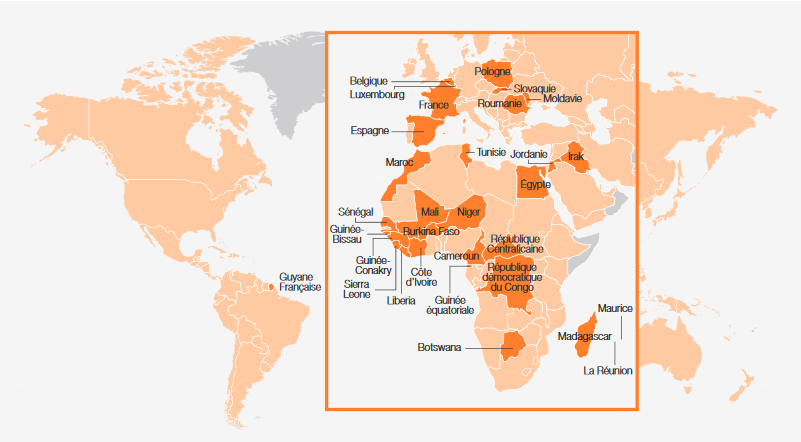
\includegraphics[scale=0.75]{./img/world_orange_2016.PNG}
    \caption{Carte des pays où est présent Orange en 2016}
\end{figure}
\paragraph*{}
Le groupe Orange est majoritairement présent en Europe et Afrique. Il est avant tout un leader de la téléphonie mobile avec un total de 202 millions de clients mobile en 2016 au niveau mondial. Orange est aussi leader dans le domaine de l’accès à Internet avec 18 millions de clients Internet haut débit fin 2016, 265 000 clients \gls{ftth} et 42 millions de clients sur la téléphonie fixe fin 2014 en France. Les pays où le groupe est le plus implanté sont la France, l’Espagne, la Pologne et la Roumanie. Depuis plusieurs années maintenant Orange essaie de se développer également en Afrique dans le domaine de la téléphonie mobile et de la finance avec Orange Money.
\paragraph*{}
Le secteur d’activité principal du groupe Orange reste les Télécommunications, en étant un opérateur téléphonique majeur en France et dans bien d’autres pays tels que la Pologne, l’Espagne, la Roumanie, Côte d’Ivoire, Égypte etc. Orange est également un fournisseur d’accès Internet et depuis quelques années élargit ses activités à la domotique, vente de contenus cinématographiques et musicaux, médical, applications bancaires etc.
\paragraph*{}
Les principaux concurrents d'Orange en France dans le domaine \gls{fai} sont principalement Free, SFR-Numéricâble, OVH, Nerim, Wifirst, Bouygues Télécoms. Et pour la téléphonie mobile ses principaux concurrents sont SFR, Free et Bouygues Télécom. Tandis qu'au niveau européen sur le domaine téléphonique et \gls{fai}, les principaux concurrents sont Deutsche Telekom, Vodafone et O2 en grande majorité.
\paragraph*{}
La branche où j’effectue mon alternance depuis 3 ans est \gls{ols}. Cette branche concerne tous ce qui touche à la recherche et au développement des produits Orange. Anciennement nommé France Télécom R\&D, puis \gls{olps} en 2007, et enfin rebaptisé \gls{ols} en 2017. Cette branche destinée à la recherche de l’ensemble du groupe Orange emploie 3500 personnes répartis à travers le monde en France, Roumanie, Inde, Tunisie, Chine. Fin 2012, le nombre de brevets déposés par Orange Labs s’élevaient à 7493. La R\&D est très importante pour Orange qui investit chaque année près de 900 millions d’euros dans ce secteur. \\

\subsection{Le contexte}
\subsubsection{Le Device Mangement à Orange}
\paragraph*{}
Mon alternance se déroule plus précisément au sein de l’équipe \gls{care}  qui s’occupe de la gestion des équipements client, c’est-à-dire du « Device Management ».
\paragraph*{}
Le concept de « Device Management » possède plusieurs définitions selon les objets ou équipements gérés, et les équipes qui le mettent en place. Pour nous, le Device Management s'articule autour de quatre axes:
\begin{itemize}
\subparagraph*{}
\item Provisioning: Active ou désactive un service pour le client sur l'équipement adéquat; Applique le bon \gls{firmwareg} selon le service souscrit; Paramètre de manière personnalisé la configuration d'un équipement donné en fonction des services.
\item Assistance: Permet de diagnostiquer à distance un incident sur l'équipement; Déclencher à distance l'exécution d'action permettant de corriger un incident.
\item Tracking: Collecte et stocke des informations sur l'ensemble du parc client.
\item Maintenance: Permet la mise à jour de \gls{firmwareg} planifiés.
\end{itemize}
\paragraph*{}
L'architecture du Device Management est découpé en deux zones détaillées comme suit : 
%Import Images
\begin{figure}[!ht]
    \center
    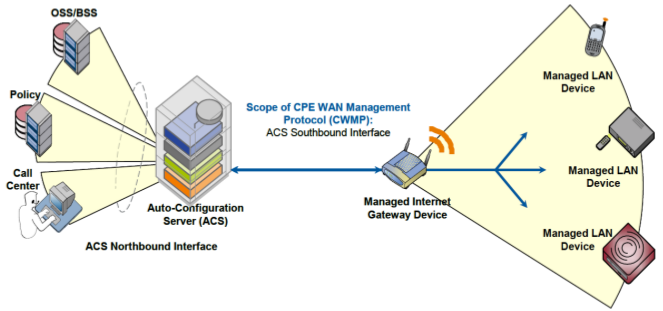
\includegraphics[scale=0.7]{./img/DM-TR-069-screen.png}
    \caption{Réseau de Device Management, côté Opérateur et côté Client}
\end{figure}
\begin{itemize}
\subparagraph*{}
\item Le coté client, où l'on retrouve le réseau privé du client, dit le \gls{lan}, avec généralement divers équipements, que l'on nomme \gls{cpe}, tels que, une passerelle Internet, un décodeur TV, un téléphone, une caméra \gls{ip}, des capteurs domotiques etc.
\item Le coté serveur, se trouvant chez Orange, où l'on va retrouver les serveurs, que l'on nomme \gls{acs}, qui vont permettre de faire ce que l'on appelle du Device Management.
\end{itemize}
\paragraph*{}
L’un des objectifs du Device Management, pour l’équipe \gls{care}, est d’apporter un service d’aide et de dépannage aux clients, tous en restant à distance. Dans le but de ne pas avoir à faire déplacer un technicien sur place, pour un problème qui peut être résolu à distance par l’exécution de scripts, lancement de tests et analyse, ou encore correction de bug. Le rôle de l’équipe \gls{care}, est de concevoir l’intégration de ces outils qui pourront être utilisés à distance.
\paragraph*{}
La supervision et la maintenance du parc Orange sont d'autres activités dans le
périmètre du domaine du Device Management. Ce parc contient les différents produits vendus par Orange et qu’Orange s'engage à maintenir. On comprend alors l'importance des activités de supervision et de maintenance. Pour gérer ce parc, Orange a besoin, entre autres, d'identifier les différents équipements présents et d'accéder à leurs  caractéristiques. Les outils de Device Management  développés au sein de l'équipe \gls{care} permettent, cette fois, de remonter aux \gls{acs} toutes les informations nécessaires pour superviser et maintenir le parc. Il permet également de mettre à jour et corriger des bugs en envoyant de nouvelles versions de \gls{firmwareg} aux équipements concernés. \\
\subsubsection{Document TR-069 et protocole normalisé CWMP}
\paragraph*{} Avant de continuer, il est important de préciser quelques élèments de vocabulaire propre au Device Management et décrire plus en détail comment \gls{acs} et \gls{cpe} communiquent.
\paragraph*{}Comme nous l'avons vu précédemment, un \gls{acs} est un serveur qui permet de manager un \gls{cpe}, et par conséquent de réaliser du Device Management sur le parc client. 
\paragraph*{}Les interactions entre \gls{acs} et \gls{cpe} sont standardisées et décritent dans le \gls{doctr069g}. Ce document permet, entre autre, de décrire comment implémenter la norme TR-069 sous la forme du protocole \gls{cwmp}, tant sur les \gls{acs} que sur les \gls{cpe}.
\paragraph*{}Ce \gls{doctr069g} est le résultat d'un consortium de plusieurs industriels. Ce consortium, appelé le \gls{bbf}, ce compose de plus d'une centaine de membres dont Orange, CISCO, Deutch Telecom, Huawei, Juniper, le gouvernement du Canada, Intel et bien d'autres. Le \gls{bbf} vise à décrire la gestion des équipements clients, dit \gls{cpe}, par les serveurs de gestion d'équipements, dit \gls{acs}. C'est par le \gls{doctr069g} que le \gls{bbf} décrit un standard permettant la communication entre \gls{cpe} et \gls{acs} pour une bonne gestion des équipements clients.
\paragraph*{}Ce standard décrit un modèle de donnée, que l'on nomme \gls{datamodelg}, comportant une partie commune pour chaque équipement implémentant le \gls{doctr069g}. Le management d'un équipement par un \gls{acs} repose en partie sur la présence de ce \gls{datamodelg}. Le standard décrit également différentes méthodes, que l'on nomme RPC Methods, obligatoire ou facultative, qui doivent être implémentées soit par l'\gls{acs} soit par le \gls{cpe}. Ces RPC Méthodes\footnote{Les principales RPC Methods des \gls{acs} et \gls{cpe} sont visibles en annexe.} vont permettre la communication entre \gls{acs} et \gls{cpe}, et ainsi rendre possible à l'\gls{acs} le managment de ses \gls{cpe}.
\paragraph*{}Plus précisément, un \gls{cpe}, afin de pouvoir échanger avec un \gls{acs}, doit implémenter le \gls{doctr069g} sous la forme d'un client \gls{cwmp}. Les échanges \gls{cwmp} sont transportés sur du \gls{http} et encapsulés dans des messages \gls{soap}. La création d'une session \gls{cwmp} ce fait toujours par le \gls{cpe}. L'\gls{acs} ne peut pas créer de session, en revanche il possède différentes techniques\footnote{Ces techniques feront l'objet de parties présentées plus loin dans le document.} lui permettant de demander au \gls{cpe} de venir initialiser une session \gls{cwmp}. \\

\subsection{Objectifs}
\paragraph*{}Au cours des trois années passées dans l'équipe \gls{care}, il m'a été confié différents objectifs d'importance et de responsabilité croissante. Ces objectifs m'ont permis de monter en compétences tant sur l'aspect technique que l'aspect transversal du métier d'ingénieur informatique.\\
\subsubsection{Première année}
\paragraph*{}À mon arrivée le principal objectif été de me faire monter en compétence sur le domaine du device management, et plus particulièrement sur le protocole \gls{cwmp}. Il a donc été décidé de me faire tout d'abord monter en compétence sur le côté client, puis sur le côté serveur, par différentes missions que nous verrons par la suite\footnote{La partie intitulée "Monté en compétence sur le protocole \gls{cwmp}" est entièrement dédié à cet apprentissage du domaine du device management et du protocole \gls{cwmp}}. \\
\subsubsection{Deuxième année}
\paragraph*{}En début de deuxième année, ayant acquis les connaissances nécessaires lors de la première année, l'objectif était de me faire développer une application permettant de réaliser une série de test de client \gls{cwmp} de manière automatique\footnote{La partie intitulée "Conception et développement de TINK" est entièrement dédiée à la réalisation de cet outil.}.
\paragraph*{}Un autre objectif de cette deuxième année a été d'encadrer un stagiaire de Master 2 Informatiques, Jean-Pierre ONA, qui devait travailler avec moi sur ce projet. Jean-Pierre a été présent de mars à aout 2016, son sujet de stage portait sur la conception et le développement d'une \gls{ihm} pour l'application de mon projet.
\paragraph*{}Enfin, l'un des objectifs de cette deuxième année était de trouver une personne pour prendre la suite du projet de test d'équipements. Pour ce faire je devais mener une activité de tutorat afin de faire monter en compétence une personne de l'équipe sur ce projet.\\
\subsubsection{Troisième année}
\paragraph*{}Pour la troisième année l'objectif était avant tous de continuer le développement et l'ajout de fonctionnalité à l'application réaliser l'année précédente, mais également de la mettre en production et d'en assurer l'aide aux utilisateurs. 
\paragraph*{}Un autre des objectifs était de prévoir mon départ en réalisant un transfert de compétence sur l'outil développé. Cela devait se faire par la rédaction de différentes documentations permettant aux futurs développeurs de continuer mon travail, ainsi que la présentation de l'outil aux équipes susceptibles de récupérer l'outil. 
\paragraph*{}De plus, cette troisième année était pour moi l'occasion de faire de la communication et des présentations de l'application à différentes équipe françaises et internationales. L'objectif était de faire connaître l'outil et d'avoir les premiers utilisateurs.\\


\newpage
\section{Monté en compétence sur le protocole CWMP}
\subsection{Études d'équipements}
\paragraph*{}Ce projet s'est déroulé tous au long de la première année. La personne avec qui je travaillais sur ce projet, Serge MARTIN, étant partie à la retraite en octobre 2015, et ayant dû me consacrer moi-même à d'autres missions, ce projet a été progressivement arrêté durant ma deuxième année. L'un des objectifs de ma deuxième année avait été de continuer ce projet le temps que l'on trouve une autre personne à former pour prendre la suite. Malheureusement, cet objectif n'a été que partiellement réalisé, faute de disponibilité de la part de la personne devant reprendre le projet, menant ainsi à son arrêt.
\paragraph*{}Le projet consiste à faire différents tests sur des équipements Orange que l’on peut retrouver côté clients. Ces tests peuvent être demandés par d'autres équipes ou bien des membres même de \gls{care}. Ces demandes sont faites lorsque l'on a besoins de savoir comment fonctionne certains équipements Orange au niveau \gls{cwmp}, connaître leurs comportements réseau dans certaines situations, ou encore récupérer une partie voir l'intégralité de leur \gls{datamodelg}. Le domaine de ces tests est très diversifié et peut prendre quelques heures, comme plusieurs semaines. \\
\subsubsection{Présentation du réseau isolé}
\paragraph*{}Afin de reproduire au mieux les conditions réelles, avoir une visibilité intégrale sur les échanges ayant lieu, et un contrôle à tous les niveaux du réseau opérateur, nous avons décidé de reproduire un réseau opérateur que l’on nomme « réseau isolé ». 
\paragraph*{}Ce réseau est constitué d’un micro \gls{dslam} faisant la jonction entre la partie opérateur Orange et les clients Orange. Il permet de gérer les « clients » en leur attribuant une adresse \gls{ip} publique via un service de \gls{dhcp} et en créant des lignes \gls{adsl} avec login et mot de passe attribués. 
\paragraph*{}Du cotés clients, on retrouve les différents types de box internet auxquels sont connectés les équipements clients, dans leur réseau \gls{lan}. 
Du coté opérateur, nous avons mis en place un serveur \gls{dhcp} pour attribuer des adresses \gls{ip} aux machines du réseau opérateur. Un serveur \gls{dns} est également présent pour la résolution des noms. Ce serveur \gls{dns} est aussi utilisé par les box internet des clients comme serveur \gls{dns} primaire. Nous avons aussi deux serveurs \gls{acs}. Un premier du même type que celui utilisé par Orange Labs pour les tests et recherches. Et un second, sous forme de \gls{servletg} Java\footnote{La servlet Java fait l'objet d'une sous-partie intitulé "Création d'un \gls{acs} Servlet", puisque j'ai également eu à travailler dessus durant ma première année} qui possède moins de fonctionnalités que le premier, mais qui est très utilisé pour les tests de comportement CWMP\footnote{Les test de comportement font l'objet de la partie intitulé "Test de comportement CWMP d'équipement"}. Vous pouvez voir ci-dessous le plan du réseau isolé que nous utilisons et qui est décrit ci-dessus.
\paragraph*{}
%Import Images
\begin{figure}[!ht]
    \center
    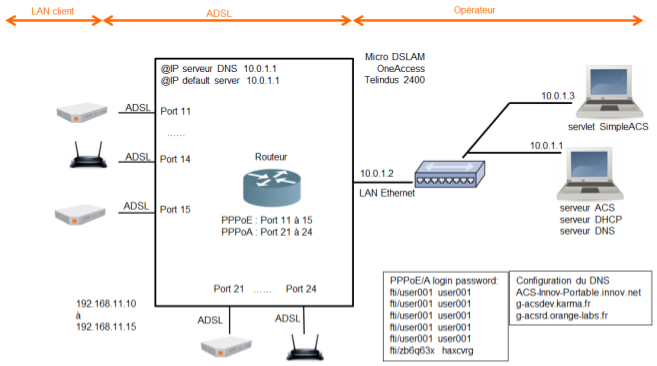
\includegraphics[scale=0.7]{./img/reseau_isole.png}
    \caption{Schéma du réseau isolé}
\end{figure}
\paragraph*{}Nous ne rentrerons pas plus en détail sur ce réseau ici. Il faut également savoir que nous avons placé un concentrateur du côté opérateur, entre les serveurs et le micro \gls{dslam} dans le but de pouvoir analyser le trafic réseau en plaçant un \gls{sniffeurreseaug} tel que Wireshark. 
\paragraph*{}Il arrive parfois que certains équipements dialoguent via \gls{https} avec le serveur \gls{acs}. Ce type de protocole sécurisé nous empêche de faire certains tests liés au protocole \gls{cwmp}, puisque nous n’avons pas les certificats nécessaires au déchiffrage des trames \gls{https}. \\
\subsubsection{Test DNS}
\paragraph*{}Au cours de la première année, une équipe a eu besoin de connaître le comportement des équipements Orange vis-à-vis de leur serveur \gls{dns}. Nous avons donc utilisé le réseau isolé afin de réaliser différents tests sur les équipements en questions.
\paragraph*{}Plus exactement, cette équipe devait migrer des serveurs \gls{acs}. Les \gls{cpe}, selon leur client \gls{cwmp} envoie des requêtes à leur serveur \gls{dns} respectif afin de connaître leur \gls{acs}. Les membres de cette équipe voulaient donc connaître l’impact, en terme de nombre de requêtes \gls{dns}, que cela allait avoir sur les serveurs \gls{dns} des équipements liés à ces serveurs \gls{acs}. Le but premier était de s’assurer que le nombre de requêtes faites par les équipements, pour connaître la nouvelle adresse \gls{ip} de leur \gls{acs}, n’allait pas faire tomber les serveurs \gls{dns} qui sont sollicités par ces équipements. 
\paragraph*{}Nous nous sommes demandés dans un premier temps, quand est ce que doivent apparaître ces requêtes \gls{dns}. Pour ce faire, nous avons regardé ce qui est préconisé par le \gls{doctr069g}, puisqu’en toute logique, les équipements qui communiquent et sont gérés par un serveur \gls{acs}, doivent respecter cette norme le plus fidèlement possible. A partir de la norme, nous avons isolé plusieurs cas d’usage où un équipement se doit de contacter son \gls{acs}, et donc avant cela, faire un appel \gls{dns} pour connaître son adresse \gls{ip}. 
\paragraph*{}Nous avons ensuite mis en place chaque équipement, dans notre réseau isolé, et les avons redirigés vers le serveur \gls{acs} et le serveur \gls{dns} appropriés pour procéder aux tests et à la vérification du respect des cas d’usages. 
\paragraph*{}Il y avait donc deux objectifs. Le premier, était de vérifier si les équipements respectent bien le \gls{doctr069g}. Tandis que le second objectif était de contrôler et relever le nombre de requêtes faites par les équipements vers leur serveur \gls{dns}. 
\paragraph*{}Après avoir testé les différents cas d’usage, sur tous les équipements, il apparaît que certains équipements ne respectent pas le \gls{doctr069g} en termes d'appel \gls{dns}. Certains cas d’usage sont tous simplement ignorés par l'équipement, ce qui représente une grave
erreur d'implémentation du \gls{doctr069g} sur ces équipements. Afin que ces erreurs soient corrigées, nous avons remonté ces anomalies au service qui veille au respect du \gls{doctr069g} et qui font les correctifs des bugs sur les équipements. Nous avons également pu donner des éléments de réponse à la première question par le biais d’un rapport des tests effectués et de présentations aux cours de réunions d'avancement. Au vu des données que nous leur avons remonté, ils ont pu déduire que l'impact du nombre de requête envoyées aux serveurs \gls{dns} ne générerait pas une surcharge des serveurs. \\
\subsubsection{Test de comportement CWMP d'équipement}
\paragraph*{}Les tests CWMP sont des tests qui nous sont demandés par notre équipe de manière irrégulière selon les besoins de l'équipe. Le but de ces tests est de connaître les caractéristiques \gls{cwmp} de ces équipements que nous utilisons. Mais aussi être capables de savoir comment ils réagissent dans différentes situations et savoir comment leur client \gls{cwmp} implémente le \gls{doctr069g}. Bien entendu, nous ne testons ici que des équipements embarquant un client \gls{cwmp} capable de communiquer avec son \gls{acs}.
\paragraph*{}A chaque fois que l’équipe récupère un nouveau device susceptible de pouvoir faire du Device Mangement, il doit faire l’objet de ces tests \gls{cwmp}. L’ensemble des résultats de ces tests sont ensuite documentés et archivés afin de pouvoir être réutilisés si besoins. Ces demandes peuvent permettre d'anticiper la venu de nouveaux équipements dans le parc client d'Orange, elles permettent de savoir si nous auront des difficultés à manager ces nouveaux équipements avec la version actuelle de \gls{karmag}. 
\paragraph*{}Le \gls{doctr069g} est extrêmement long et décrit l'ensemble des régles qu’un \gls{cpe} se doit d'implémenter, avec plus ou moins de rigueur dans certain cas. Pour tester les équipements que nous recevons, il a été décidé de regarder le respect de 4 points qui sont les plus importants pour les travaux fait dans l’équipe. Ces quatre points\footnote{Nous ne rentrerons pas dans le détail technique de ces quatre tests} ont été sélectionnés pour être testés systématiquement car ce sont ceux qui sont le plus souvent demandés par les membres de l’équipe. Un cinquième point a été rajouté récemment avec la création et l’ajout dans le réseau isolé de l’ACSServlet\footnote{Voir la partie intitulé "Création d'un ACS Servlet"}. Ce cinquième test que j’ai pu rajouter consiste à extraire l’intégralité du \gls{datamodelg} d’un équipement. L’extraction du \gls{datamodelg} d’un équipement fait souvent l’objet de demande externe, et fait appel à des fonctionnalités \gls{cwmp} qui sont intéressantes à être testées pour chaque équipement.
\paragraph*{}Pour procéder aux tests, il faut avant tout pouvoir placer les équipements dans notre réseau isolé, ce qui nécessite parfois sa configuration. Les améliorations et modifications peuvent être faites à plusieurs niveaux. Cela peut être une modification de la configuration du micro \gls{dslam}, ajouter de nouveaux types de connections\footnote{Les équipements que nous avons peuvent communiquer soit par PPPoE soit par PPPoA, cela nécessite la configuration de port dédiés à ces deux types de connections.} au micro \gls{dslam}, rajouter des plages d’adresses sur le serveur \gls{dhcp}, ou bien encore créer de nouveaux domaines dans la configuration du serveur \gls{dns}.
\paragraph*{}Cependant, il arrive que l’ajout de l’équipement dans notre réseau isolé ne soit pas possible. Soit à cause de critères physiques, comme on a pu le rencontrer avec des dispositifs 4G Huawei, auquel cas nous ne pouvons pas procéder à certains tests, voir à l’intégralité des tests. Soit, à cause de contraintes techniques, qui nous empêchent de pouvoir faire le moindre test. Cela arrive lorsque l’équipement utilise un certificat \gls{ssl}, que nous ne possédons pas, dans ce cas aucuns des tests ne sont possibles.
\paragraph*{}De manière générale, les 4 principaux tests sont faits à partir de scripts JavaScript exécutés depuis le serveur \gls{acs}\footnote{C'est ce serveur même qui est utilisé pour la recherche et l'anticipation.} vers lequel remontent les équipements dans le réseau isolé. Tandis que le cinquième test est fait en redirigeant l’équipement vers l’ACSServlet. Lorsque nous rencontrons un problème avec un équipement, empêchant son installation dans le réseau isolé, nous faisons les tests sur le réseau public. Mais cela rend les tests plus longs et compliqués. Il faut parfois trouver de nouvelles façons de faire et cela ne suffit pas toujours rendant parfois des tests impossibles. \\
\paragraph*{}Ce projet s'est déroulé lors de ma première année. L'étude d'équipements aussi bien comportement \gls{cwmp} que \gls{dns}, la mise en place du réseau isolé et la restitution sous forme oral et écrite des rapports de test, m'auront permis d'acquérir de solides bases sur le protocole \gls{cwmp}, et une excellente entrée en matière dans le Device Management. Cela m'aura également permis de renforcer mes compétences en Système et Réseaux, particulièrement sur la configuration de serveur \gls{dns} et \gls{dhcp} Mais aussi dans tous ce qui est protocole de communication et gestion d'OS. Enfin, cela m'aura permis de renforcer mes compétences en rédaction et présentation orale.\\
\subsection{Étude de client CWMP}
\paragraph*{}Afin de rentrer plus en profondeur sur les spécificités d'implémentation du \gls{doctr069g} pour un \gls{cpe}, j'ai étudié lors de ma première année deux clients \gls{cwmp}. L'étude de ces clients \gls{cwmp} avait pour objectif de déterminer quel pouvait être les clients susceptibles d'être réutilisés par des équipements du parc Orange, afin de faciliter leur management par \gls{karmag}.
\paragraph*{}Actuellement tous les constructeurs d’équipement n’implémentent pas
systématiquement un client \gls{cwmp} sur leurs équipements. Cela rend impossible le device management lorsqu’un client achète un équipement chez un de ces constructeurs. Or, Orange s’engage à pouvoir manager l’ensemble des équipements connectés à la LiveBox du client. Par conséquent, nous avons décidé de fournir ce que l’on appelle un « toolkit \gls{cwmp} », qui aurait pour but d’aider les constructeurs qui le souhaitent, à implémenter sur leurs équipements un client \gls{cwmp}. Ce client serait certifié par Orange comme étant capable de communiquer avec nos serveurs \gls{acs}, et donc être managé. La question qui s’est donc posée, était de savoir ce que contiendrait le toolkit proposé par Orange. Pour cela, nous avons procéder à la comparaison de clients \gls{cwmp}. \\
\subsubsection{Client EasyCWMP}
\paragraph*{}L’objectif était de voir dans un premier temps si dans le domaine de l’open source il existe des clients \gls{cwmp} qui ont été développés. Puis, après avoir listé les différents clients \gls{cwmp} open source, je devais récupérer et tester ceux qui semblaient les plus prometteurs et qui implémentent le plus fidèlement le \gls{doctr069g}.
\paragraph*{}Afin de correctement comparer les différents clients open source, et vérifier qu’ils respectaient bien le \gls{doctr069g}, j’ai lu l’intégralité du \gls{doctr069g} écrite par le \gls{bbf}. Cela m’a permis de monter rapidement en compétence sur le sujet. De plus, la norme étant rédigée en anglais cela m’a également permis de monter en compétence sur l'anglais technique.
\paragraph*{}La comparaison entre les clients open source trouvés ne s'est pas faite uniquement sur le respect de l'implémentation du \gls{doctr069g}. Le logiciel devait être régulièrement tenu à jour, et le projet open source devait être encore "vivant", c'est à dire que la communauté derrière le développement du client devait être active. Il a donc fallu s'intéresser plus en détail sur la provenance des clients, vérifier qu'une documentation était présente et à jour, ainsi que regarder la date des dernières versions des clients sélectionnés.
\paragraph*{}A la suite de cette comparaison théorique des différents clients \gls{cwmp} que j’ai pu identifier, il a été décidé de n’en récupérer qu’un seul, nommé EasyCWMP et développé en C par l’entreprise PIVA Software. Seul le code source est disponible sur leur site. Les documentations d’installations et de spécifications n’étaient pas accessibles librement. Pour les récupérer il faut les commander, et donc les payer à PIVA Software, mais nous n'avons pas jugé cela comme étant un frein.
\paragraph*{}Nous nous sommes intéressés à ce client \gls{cwmp} open source car il est le seul à implémenter toutes les méthodes dites obligatoires du \gls{doctr069g}, contrairement aux autres clients open source rencontrés qui ne les implémente jamais toutes. De plus, nous avons pu voir qu’il était très régulièrement mis à jour. Bien entendu cela était purement théorique à ce moment puisque nous n'avions pas encore pu tester le client en question.
\paragraph*{}Nous possédons pour la recherche et l'anticipaition un \gls{acs}, nommé g-acsdev, afin d'évaluer et réaliser certains tests en ligne sur les clients qui nous semblent intéressants. Cet \gls{acs} est développé par l'entreprise Arris. C'est ce même type d'\gls{acs} qui est présent dans le réseau isolé. Ainsi, après avoir récupéré le code du client EasyCWMP, l’objectif était de l’installer sur un PC afin de le faire se connecter à g-acsdev.
\paragraph*{}L’une des difficultés a été de l’installer sans avoir de documentation, d’autant plus que c’était la première fois que je devais réaliser ce type d’installation en compilant le programme et en installant toutes les libraires dépendantes entre elles. Cela m’a permis de monter en compétence en C puisque je devais comprendre comment compiler le client C avec ses différentes librairies. Puis comprendre comment lancer le client, modifier sa configuration, utiliser les différentes méthodes \gls{cwmp} qu’il implémente pour vérifier leurs bon fonctionnement, et enfin le faire communiquer avec g-acsdev. Toutes ces étapes de compilation, configuration et test, ce sont faites sur une machine linux. Une partie du code du client était en Shell, ce qui m’a permis de monter en compétence en Unix également. Mon tuteur m’a expliqué de nombreux aspects de C et de Shell afin de comprendre au mieux le code du client.
\paragraph*{}Après avoir réussi à faire communiquer parfaitement le client EasyCWMP avec g-acsdev et avoir testé les méthodes \gls{cwmp} qu’il implémente, il m’a été demandé de modifier le code du client. L’objectif était de rajouter des paramètres dans son \gls{datamodelg} et de voir ces modifications apparaître dans l’interface web de g-acsdev lorsque l'on explorerait son \gls{datamodelg}. Cela m’a permis de rentrer plus en détail dans le code du client, puisque rajouter des branches au \gls{datamodelg} implique de modifier le code du client à différents niveaux. Tant au niveau C que Shell, j’ai dû comprendre comment le logiciel était codé, la relation entre les différents fichiers et appels de librairie. Ce qui m’a également permis de monter de nouveau en compétence en C mais également d’apprendre à comprendre un code que l’on récupère, le tout sans aucune documentation.
\paragraph*{}Cette activité m’aura donc apporté énormément dans plusieurs domaines techniques tels que le C, le Shell et renforcer ma monter en compétence sur le protocole \gls{cwmp}. Elle m’aura également permis de voir comment se déroule une activité de bout en bout de manière totalement autonome. A la fin de l’activité il m’a également été demandé de créer une documentation sur l’installation des différents prérequis et du client EasyCWMP même, ce qui m’a permis d’apprendre à rédiger une documentation. De plus, le fait d’avoir fait des recherches dans le domaine de l’open source, m’a aidé à mieux comprendre l’open source avec ses différentes normes et licences, les projets collaboratifs etc. Enfin, cette activité m’aura permis de véritablement rentrer dans le device management et de mieux comprendre le côté client. \\
\subsubsection{Comparaison EasyCWMP et tr69agent}
\paragraph*{}Nous avons dégagé quatre propositions de contenu du toolkit. Ces quatre propositions de contenue du toolkit ne pourront pas être décrites ici. Afin de départager ces différentes possibilités de contenu nous devions apporter des éléments de comparaison. Par ailleurs, ce n’est pas nous qui avons pris la décision finale, mais les responsables de HomeService\footnote{HomeService correspond au service en-dessous d'\gls{ols}.} qui à partir de cette étude ont pu prendre une décision sur la stratégie à adopter.
\paragraph*{}Ces propositions ont amené à comparer le client EasyCWMP au client nommé tr69agent. Ce client \gls{cwmp} a été développé par Orange. Bien que nous possédions l’intégralité de la documentation et des droits liés à ce logiciel, nous devions vérifier s’il était plus avantageux que le client proposé par PIVA Software. Mon rôle dans cette étude a donc été de comparer ces deux clients et ainsi déterminer quels sont les points faibles et points forts de chacun de ces deux clients.
\paragraph*{}Pour ce faire je leur ai fait passer les tests de comportement \gls{cwmp} et tests \gls{dns}. Les deux clients ont été installés dans des environnements identiques afin de ne pas perturber les résultats. L’analyse de ces tests n’a pas permis de départager les deux clients. En revanches, aucun des deux ne les satisfaisaient complétement, ce qui impliquait que peu importait le client qui serait choisi, il faudrait le retravailler afin de le rendre parfaitement en adéquation avec le \gls{doctr069g}.
\paragraph*{} Je suis donc rentré plus en détails dans la comparaison, et j’ai regardé du côté de leurs caractéristiques. Tels que, le poids du logiciel après installation, le langage de programmation utilisé, la clarté de leur code, et les méthodes \gls{cwmp} obligatoires et facultatives implémentées.
\paragraph*{}En dehors de cet aspect technique de comparaison des deux clients, j’ai pu voir comment mener une étude, présenter des résultats et préparer leurs présentations. De plus, j’ai rédigé un rapport sur l’ensemble des tests de comparaison des deux clients, ce qui m’a permis de m’exercer sur l’aspect rédactionnel. Je n’ai malheureusement pas pu assister à la présentation finale puisque cela s’est produit lors de l’une de mes périodes de cours, mais j'ai pu participer à la préparation de la présentation et du support. \\
\subsubsection{Résultats}
\paragraph*{}À la suite de la comparaison entre les client \gls{cwmp} EasyCWMP et tr69agent, une des quatre propositions a été retenue. Cette solution consiste, entre autre, à fournir au sein du toolkit le client tr69agent, une documentation permettant l'intégration du client, ainsi qu'une plateforme de test\footnote{La réalisation de cette plateforme fait l'objet de la partie suivante, intitulé "Conception et développement de TINK"} d'implémentation de client \gls{cwmp}. 
\paragraph*{}Les études de ces deux clients m'auront permis de renforcer mes compétences sur le protocole \gls{cwmp}, en particulier sur le côté client. Mes compétences rédactionelles auront également été renforcées. \\
\subsection{Création d'un ACS Servlet}
\paragraph*{}Après être monté en compétence sur \gls{cwmp} et avoir travaillé du côté client du device management avec EasyCWMP et tr69agent, j’ai travaillé du côté serveur. Ce projet s'inscrit encore une fois dans le courant de ma première année.
\paragraph*{}Dans le cadre des tests d'équipements, nous avions besoin d’un deuxième \gls{acs} dans le réseau isolé afin d’effectuer certain tests. C’est pourquoi, un des membres de l’équipe a conçu ce que l’on appelle une \gls{servletg}. Cette \gls{servletg} est codée en langage Java, et se comporte au sein du réseau isolé comme un serveur \gls{acs}. La \gls{servletg} s’installe sur un serveur web installé sur un PC du réseau isolé, permettant ainsi d’avoir un équivalent de serveur \gls{acs} mais extrêmement minimaliste.
\paragraph*{}L’avantage d’avoir une \gls{servletg} comme \gls{acs} est que l’on peut y rajouter les fonctionnalités dont nous avons besoin. Elle est également facile à installer, puisqu’il suffit uniquement d’un serveur web.
\paragraph*{}On m’a donc demandé de reprendre la \gls{servletg} déjà faite et de l’améliorer afin que dans un premier temps elle puisse extraire le \gls{datamodelg} d’un équipement qui viendrait dialoguer avec elle. Par conséquent, elle devait aussi pouvoir communiquer avec un maximum d'équipements qui implémentent le \gls{doctr069g}. A l’origine, la \gls{servletg} qui a été développée ne pouvait communiquer qu’avec un nombre restreint de types d'équipements à cause de contraintes techniques que je devais donc résoudre.
\paragraph*{}
%Import Images
\begin{figure}[!ht]
    \center
    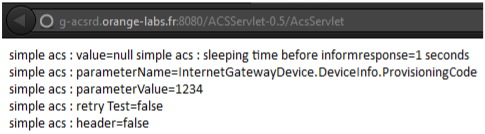
\includegraphics[scale=0.9]{./img/acs_servlet_05.png}
    \caption{Affichage web de l’ACSServlet-0.5, ancienne version}
\end{figure}
\paragraph*{}Comme on peut le voir ci-dessus, la dernière version de la \gls{servletg}, nommé « ACSServlet-0.5 » était extrêmement minimaliste en termes d'affichage. L'état des paramètres utilisés pour les tests d'équipements était modifié via l’url et aucune vérification n’était faite sur la cohérence des valeurs entrées. Par ailleurs, elle implémentait un nombre limité de méthodes \gls{cwmp}. Je devais donc améliorer l’interface web afin de proposer une solution plus simple pour modifier les paramètres. De plus, j’ai pensé qu’un contrôle des valeurs de ces paramètres serait un plus et une sécurité pour l’utilisateur. Le tout devait bien entendu pouvoir fonctionner avec le plus grand nombre de device possible en implémentant davantage de méthodes \gls{cwmp}. Enfin, elle devait pouvoir extraire systématiquement le data model de l’équipement dans un fichier au format .csv.
\paragraph*{}Comme pour les précédentes activités, j’étais libre de procéder dans l’ordre que je souhaitais pour réaliser ce travail. L’objectif étant là encore de me faire gérer de bout en bout une activité, découper les différentes tâches et étapes, le tout sans hésiter à aller voir les personnes susceptibles de m’apporter des informations et explications dans les domaines dont j’avais besoin.
\paragraph*{}J’ai tout d’abord cherché à comprendre le code de la \gls{servletg} que l’on m’avait donné. N’ayant pas vraiment de connaissance dans le langage Java, je devais également monter en compétence dans ce domaine. Cela m’a pris plusieurs jours pour voir et comprendre le code, les fonctionnalités mises en place, ainsi que les outils utilisés pour développer la \gls{servletg}.
\paragraph*{}Je me suis familiarisé avec le code en ajoutant des méthodes \gls{cwmp} qu’un serveur \gls{acs} doit avoir pour communiquer avec différents équipements. J’ai pu identifier et implémenter ces différentes méthodes depuis le \gls{doctr069g}, mais également en analysant les échanges de trames sur le réseau isolé entre un équipement et son \gls{acs}. L’implémentation de ces méthodes m’a permis de me familiariser plus rapidement avec l’ensemble du code. J’ai également pu avoir plusieurs explications de la personne qui a développé les premières versions de la \gls{servletg}.
\paragraph*{}Une fois cette première étape de découverte passée, j’ai pu faire communiquer la \gls{servletg}, avec ces nouvelles méthodes, au client EasyCWMP sur lequel j’avais travaillé précédemment. Et ainsi vérifier son bon fonctionnement sur un premier type d’équipement.
\paragraph*{}J’ai part la suite réfléchi à la méthode à employer pour réaliser l’extraction du \gls{datamodelg} d’un équipement quelconque. Un \gls{datamodelg} ce présentant sous forme d’un arbre. Je me suis donc renseigné sur les différents types de parcours d’arbre possible et algorithme associé, afin de choisir le plus optimisé, mais aussi le plus en adéquation avec les contraintes techniques que j’avais. Le \gls{datamodelg} devait être extrait sous forme d’un fichier .csv afin de faciliter sa réutilisation et lecture par la suite.
\paragraph*{} Une fois l’implémentation de cet algorithme fait, j’ai cherché à le tester sur un maximum d’équipements. Il fallait donc modifier la \gls{servletg} de telle façon à ce qu’elle puisse s’adapter à l’équipement qu’on lui présente en entrée, et communiquer avec. Cela a été assez compliqué et partiellement réalisé, puisque tous les équipements ne dialoguent pas forcément de la même façon, et apporte donc régulièrement de nouvelles contraintes. Les versions \gls{cwmp} peuvent différer selon les équipements, modifiant alors les en-têtes des trames. Il se peut également que certaine informations dans le corps de la trame ne soit pas présentes d'un équipements à l'autre selon l'implémentation de \gls{cwmp} qu'ils ont.  Ce travail d’adaptation de la \gls{servletg} à un équipement nécessiterait beaucoup plus de temps que celui disponible pour l’activité entière.
\paragraph*{}Après avoir permis à la \gls{servletg} de communiquer avec différents équipements et d’extraire leur \gls{datamodelg}, j’ai voulu faire des tests d’extraction de \gls{datamodelg}. L’objectif était de comparer le temps d’extraction du \gls{datamodelg} de plusieurs équipements depuis ma \gls{servletg}, avec le temps d’extraction depuis un script JavaScript exécuté sur le serveur \gls{acs} g-acsrd. Ces mesures ont été réalisées selon différents critères tels que, le nombre de paramètres (feuille), le nombre de groupe de paramètre (branche), le poids final du \gls{datamodelg} dans un .csv et l’équipement dont le \gls{datamodelg} est extrait \footnote{Les capacités de RAM et cpu de l'équipement sont très influentes sur l'éxecution des requêtes permettant de parcourir le \gls{datamodelg}}. Cela m’a amené à optimiser mon algorithme d’extraction, et plus généralement le code entier de ma \gls{servletg}.
\paragraph*{}Une fois l’étape d’optimisation du code effectué, j’ai créé une page d'accueil de la \gls{servletg} en html et css avec un formulaire pour modifier les paramètres plus simplement. De plus, lors de l’envoi des valeurs des paramètres, j’ai rajouté une vérification afin de détecter différentes anomalies ou valeurs impossibles qui seraient entrées par l’utilisateur et entraineraient un blocage de l’équipement.
\paragraph*{}Enfin, après avoir testé le bon fonctionnement de la \gls{servletg}, j’ai pu l’installer sur le serveur g-acsrd et donc la rendre accessible depuis l’extérieur, comme on peut le voir ci-dessous.
\paragraph*{}
%Import Images
\begin{figure}[!ht]
    \center
    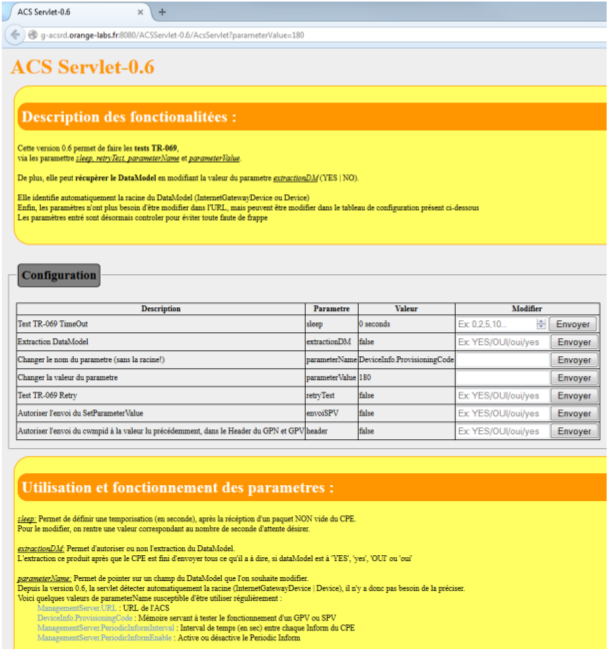
\includegraphics[scale=0.74]{./img/acs_servlet_06.png}
    \caption{Affichage web de l’ACSServlet-0.6, nouvelle version}
\end{figure}
\newpage
\paragraph*{}J’ai également ajouté une partie sur la page d'accueil expliquant les fonctionnalités et le rôle de cette \gls{servletg}, avec des exemples de valeurs attendues pour les paramètres et une note d'explication pour chacun d’eux.
\paragraph*{}Cette activité m’aura permis de monter en compétence en Java, plus particulièrement du côté \gls{servletg}. Mais également de m’améliorer dans la gestion d’une activité de plusieurs mois entre-coupé par les périodes de cours et les autres activités. Enfin, j’ai pu de nouveau monter en compétence sur \gls{cwmp}. \\
\subsection{Impact sur mon parcours}
\paragraph*{}Comme nous avons pu le voir tous au long de cette partie, les activités réalisées durant la première année de mon alternance m'ont permis de monter rapidement en compétence sur le protocole \gls{cwmp}, et permis d'avoir une bonne vision du domaine du device management. La lecture du \gls{doctr069g}, puis l'activité de test d'équipements réalisée sur l'ensemble de la première année, m'ont permis de comprendre et voir différentes implémentations du protocole \gls{cwmp} et comportement d'équipements. Le projet d'étude du client EasyCWMP, puis la comparaison avec le client tr69agent, m'ont permis de rentrer plus en profondeur sur les aspects clients du protocole, mais aussi de développer des compétences en développement et génie logiciel. Enfin, le projet d'\gls{acs} \gls{servletg}, m'a quant à lui permis de rentrer plus en détails sur l'implémentation de la partie serveur du protocole. J'ai par ailleurs pu travailler avec une grande partie des membres de mon équipe durant ces projets, me permettant ainsi de m'intégrer au mieux au sein de mon service et de mon entreprise. 
\paragraph*{}Sur les domaines techniques, j'ai pu renforcer mes compétences en administration réseaux et système développées durant mon DUT R\&T. Plus précisément, j'ai consolidé les compétences sur la configuration de serveur \gls{dns} et \gls{dhcp} lors des études de comportement de client. J'ai pu également acquérir des bases de développement en C et Java dont je n'avais que très peu de notion avant mon arrivée. Ces bases en développement, comme nous le verrons par la suite, ont été extrêmement utiles et sollicitées durant la suite de mon alternance. De plus, mes compétences acquises en entreprise sur le domaine logiciel, ont pu être renforcées par les cours de développement et le projet Java de première année effectué à l'école. 
\paragraph*{}Sur les domaines transversaux, j'ai pu acquérir de solide base en rédaction de documentation et rapport d'étude. Ces documents ont été rédigés en français, mais cela m'a permis d'avoir connaissance du rendu attendu pour ces différents types de documents. J'ai également pu acquérir, grâce au projet de test d'équipements, des compétences sur les aspects de travail collaboratif. Enfin, le fait d'avoir eu une très grande autonomie sur l'ensemble des projets m'a permis de renforcer mes compétences en gestion du temps, planification et organisation de projet. Là encore, ces compétences seront grandement sollicitées et renforcées par la suite.
\paragraph*{}Ainsi, ces projets n'auront pas uniquement servi à conforter mes compétences sur le protocole \gls{cwmp} et le domaine du device management. Ils m'auront aussi permis d'acquérir des compétences transversales tel que la gestion de projet ou encore la connaissance d'entreprise.\\


\newpage
\section{Conception et développement de TINK}
\subsection{Contexte}
\paragraph*{}L’\gls{acs} que nous utilisons en production pour manager le parc client d'Orange se nomme \gls{karmag}. Il a été développé en Java par des équipes internes Orange. Il respecte l’ensemble des parties obligatoires du \gls{doctr069g} et une majorité des parties optionnelles. Les trames \gls{cwmp} qu’il reçoit sont modifiées pour s’adapter au fonctionnement interne de \gls{karmag}. De même, lorsqu’il répond à un équipement, ses messages sont créés de manière à être compris par l’équipement en question. 
\paragraph*{}Actuellement, les constructeurs d’équipements, souhaitant produire des
équipements manageables, implémentent leur propre client \gls{cwmp} sur leurs appareils. Lorsqu’ils veulent vérifier leur bon fonctionnement pour le management par Orange, ils prennent contact avec Orange pour leur faire passer une série de tests validant, ou non, la bonne communication entre l’équipement du constructeur et \gls{karmag}. Cependant, de nombreux constructeurs contactent Orange avec des embryons de client \gls{cwmp}, ne pouvant parfois pas émettre les requêtes \gls{cwmp} obligatoires du \gls{doctr069g}, y compris les requêtes les plus basiques. Ceci fait perdre un temps considérable à l’équipe en charge de ces tests. Les tests sont alors refaits, après modification du client par le constructeur, jusqu’à ce que le client \gls{cwmp} soit finalement jugé apte à communiquer avec \gls{karmag}. Cette demande de renouvellement des tests implique également un coût financier non négligeable aux équipes d’Orange. Cela pose donc un problème, puisque certains constructeurs ne pouvant pas être autonomes pour réaliser les tests sont obligés de prendre contact avec nos équipes régulièrement pour tester leurs équipements.\\
\paragraph*{}Ainsi, \gls{tink} se propose de résoudre ce problème, en permettant aux
constructeurs d’être plus autonomes dans les tests de leurs équipements avant de les
présenter pour les tests plus poussés. Pour ce faire, \gls{tink} est une plateforme accessible sur internet. Chaque constructeur peut s'y créer un compte, ajouter ses équipements, puis lancer une série de test sur les équipements de son choix. Les tests présents sur \gls{tink} n'ont pas vocation à remplacer ceux fait par les équipes interne d'Orange, mais ils doivent permettre de vérifier que l'équipement sera capable de supporter des tests plus approfondi sur son implémentation du protocole \gls{cwmp}. De même, afin d'être le plus fidèle à \gls{karmag}, \gls{tink} utilise son module permettant de dialoguer en \gls{cwmp} avec les équipments. 
\paragraph*{}Le module de \gls{karmag} permettant la traduction du protocole \gls{cwmp}, se nomme \gls{x69g}. Ce module permet ainsi de générer des trames correctement construites au niveau \gls{cwmp} à destination des équipements, tout en contrôlant que celles reçues des équipements sont compréhensibles et correctement formées pour l’instance de \gls{karmag} déployée en production. \\
\subsection{Présentation}
\paragraph*{}Il a été décidé durant le premier semestre 2015, à la suite de l'étude comparative entre les client EaysCWMP et tr69agent, de proposer un toolkit \gls{cwmp}  afin d’aider les constructeurs à implémenter un client \gls{cwmp} compatible \gls{karmag} sur leurs équipements. Les différentes solutions de toolkit \gls{cwmp} proposables ont fait l’objet d’une étude lors de ma première année. Cette étude a permis d’aboutir à la décision de proposer un toolkit \gls{cwmp} comportant le client \gls{cwmp} tr69agent développé par Orange et mis en Open Source, ainsi qu’une plateforme en ligne de test de client \gls{cwmp}. Ainsi, le constructeur aura le choix entre utiliser notre client \gls{cwmp} pouvant communiquer avec \gls{karmag}, ou bien développer son propre client \gls{cwmp} et le tester avec notre service de test en ligne. Bien entendu, ce service de test de client \gls{cwmp} n’a pas vocation à remplacer la procédure de tests effectuée par Orange, il servira à réaliser une première vérification, sans pour autant exécuter les tests plus complexes. Par la suite, l’équipe de test d’Orange sera sûre que le client qu’on leur apporte satisfait une majeure partie de ce qui est exigé.
\paragraph*{}Ce projet de conception et réalisation d’un service de test \gls{cwmp} a donc débuté en Octobre 2015, il m'a accompagné tout au long de ma deuxième, puis de ma troisième année.
\paragraph*{}D'octobre 2015 à mars 2016 nous étions trois à travailler sur le projet,  puisque comme nous allons le voir plus tard, la solution technique n’était pas encore choisie, il n’y avait donc pas la nécessité d’une personne supplémentaire. Initialement, il y avait Marc DOUET, Matthieu ANNE et moi-même, puis en mars 2016, Jean-Pierre ONA, stagiaire encadré par Matthieu ANNE, nous a rejoints afin de développer un portail web pour \gls{tink}. Puis, à partir d'aout 2016 Jean-Pierre ONA a fini son stage, nous sommes donc repassés à trois jusqu'à aujourd'hui.
\paragraph*{}Nous avons opté pour une gestion du projet de type agile durant la présence de Jean-Pierre ONA. Le fait que ma présence soit discontinue a rendu le déroulement du projet très complexe à gérer. Par conséquent, l’organisation du projet a dû être revue au fur et à mesure, ce qui convient à la gestion de projet agile. Pour Jean Pierre ONA et moi-même, c’était la première fois que nous mettions en pratique la gestion de projet en agilité, ce qui m’a permis de monter en compétence sur ce type de gestion de projet. 
\paragraph*{}À la suite de la fin du stage de Jean-Pierre ONA, nous nous sommes de nouveau retrouvé à trois sur le projet. Il nous a fallu recupèrer le travail effectué par Jean-Pierre ONA sur l'\gls{ihm} du portail web afin de pouvoir, le moment venu, le faire évoluer.
\paragraph*{}Dans ce projet, Jean-Pierre ONA et moi-même avions les rôles de concepteurs développeurs, puisque nous avons défini et réalisé l’architecture du logiciel ; mis en place et configuré l’environnement de déploiement ; et enfin développé l’intégralité du service. Matthieu ANNE a eu le rôle de Product Owner en ayant une vision globale du produit final non seulement par sa participation aux choix d’architecture logicielle, mais aussi en priorisant les différentes tâches. De plus, il s’est occupé de tenir à jour l’avancement du projet sur la plateforme de gestion interne à Orange, en ajoutant les différents \gls{userstoriesg}, \gls{sprintg} et \gls{releaseg} définis lors des réunions. Marc DOUET a supervisé le déroulement du projet et participé avec moi-même au choix de la solution technique dont fait l’objet la prochaine partie. \\

\subsection{Déploiement}
\paragraph*{}Sachant que \gls{tink} se veut être une solution d'automatisation de test en ligne, il nous a fallu chercher une solution d'hébergement. Pour la suite du document, il est important d'expliquer et apporter des précisions sur cette solution de déploiement qu'est \gls{kermitg}. \\
\subsubsection{Qu'est-ce que Kermit ?}
\paragraph*{} \gls{kermitg} est un projet interne à Orange, basé sur l'outil OpenShift de RedHat Enterprise. Ce projet interne Orange consiste à aider les développeurs dans leur cycle agile, en fournissant une plateforme de \gls{paas} permettant de faire rapidement de l'intégration et du déploiement continue. 
\paragraph*{}Les solutions \gls{paas} sont avant tous des solutions d'infrastructure cloud. Le fait que les applications soient hébergées dans le cloud offre la possibilité d'avoir un accès rapide et simple aux ressources physiques, et de pouvoir réduire ou augmenter les ressources de calcul à moindre coût. De plus, la solution de \gls{paas} se basant sur les conteneurs \gls{dockerg}, cela permet une meilleur isolation des applications, ainsi qu'une simplification du déploiement de celles-ci. L'utilisation de \gls{dockerg} encourage également les développeurs à faire des mircro services. Enfin, l'ensemble des bénéfices apportés par les solutions \gls{paas} permettent de favoriser le DevOps.
\paragraph*{}On peut donc rapidement déployer notre application de manière automatique, dans différents langages de programmation, le tout basé sur la solution de conteneurisation \gls{dockerg}. Ces conteneurs sont facilement instanciables soit via une \gls{ihm} en ligne, soit avec un outil en ligne de commande. Les conteneurs sont orchestrés et gérés par l'outil Kubernates, ce qui est transparent pour nous. \\
\subsubsection{Environnement}
\paragraph*{}L'environnement de \gls{kermitg} se compose de plusieurs éléments. L'ensemble des conteneurs reposent sur une couche physique commune. Sur cette couche physique, vient se placer se que l'on appel des "nodes". Les nodes fournissent un environnement d'exécution aux conteneurs. Ils possèdent les services requis à l'exécution de \gls{dockerg}, Kubernates et tout autre service de proxy. Enfin, dans les nodes nous avons ce que l'on appelle les "pods". C'est dans les pods que les conteneurs sont instanciés. Un pod peut contenir un ou plusieurs conteneur, il représente un hôte. On peut retrouver cet environnement sur la figure de l'architecture simplifié de \gls{kermitg} ci-dessous. 
%Import Images
\begin{figure}[!ht]
    \center
    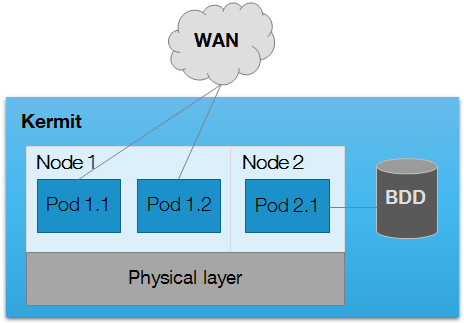
\includegraphics[scale=0.86]{./img/archi_kermit.png}
    \caption{Architecture simplifiée de \gls{kermitg}}
\end{figure}
\paragraph*{}Les données devant être sauvegardées, telles que les données d'une base de données, sont stockées sur des disques dits persistants, en dehors de la solution de \gls{paas}.
\paragraph*{}Il est important de noter que chaque pod possède sa propre adresse \gls{ip} publique. De même, nous pouvons créer autant d'\gls{url} que l'on souhaite pour chacune de ces adresses \gls{ip}. Les \gls{url} pouvant être sécurisées par l'ajout de son propre certificat, ou bien en utilisant celui déjà existant de \gls{kermitg}. 
\paragraph*{}L'utlisation de \gls{kermitg} pour pouvoir faire de l'intégration continue m'a permis de renforcer mes compétences en conteneurisation. J’ai été amené à
développer des scripts d’installation pour leur client sur des machines Linux, puisque
jusqu’à présent il n’y avait pas d’installation du client de \gls{kermitg} sur Linux. Cela m’a permis de renforcer mes compétences de scripting Linux.
\paragraph*{}Bien que je connaissais déjà \gls{dockerg} grâce à mon auto formation faite suite au projet de deuxième année de l’école, la prise en main de \gls{kermitg} m’a permis de renforcer mes compétences sur la conteneurisation et particulièrement sur \gls{dockerg}. \\
\subsection{Travail de préparation} 
\subsubsection{Recherche de solution technique}
\paragraph*{}Avant la phase de réalisation il a fallu identifier les différents choix techniques possibles, puis en choisir un selon nos besoins, tout en comprenant son fonctionnement. Cette première phase du projet s’est déroulée d’octobre 2015 à mi-janvier 2016.
\paragraph*{}Le but de cette phase était de trouver une solution technique qui répond
aux besoins de \gls{tink} tout en comprenant comment l’exploiter. Les besoins identifiés pour le projet \gls{tink} sont de permettre aux constructeurs d’avoir un accès libre à un service de test reproduisant le comportement de \gls{karmag}, sans pour autant donner un accès à \gls{karmag} même. Ainsi, les choix techniques devaient porter intégralement sur le choix du ou des module(s) \gls{karmag} à utiliser, dans quelle version et de quelle branche, puisque comme nous le verrons \gls{karmag} possède différentes branches versionnées.
\paragraph*{}Le choix d’une solution technique devait permettre à \gls{tink} de remplir au mieux ses objectifs, de pouvoir cadrer l’environnement de déploiement de la solution, ainsi que donner une direction pour la réalisation du projet en lui-même. Ce choix avait une très grande importance pour la suite du projet, puisque de lui dépendait la manière donc le projet serait réalisé, les contraintes qui seraient établies, mais également les difficultés qui allaient être rencontrées. La compréhension de la solution choisie, devait permettre la mise en place d’une première version de \gls{tink} lors de la deuxième phase du projet.
\paragraph*{}\gls{karmag} est divisé en deux branches logicielles, qui sont elles-mêmes divisées en plusieurs versions. Les deux branches, \gls{karmafrg} et \gls{karmabug}, offrent les mêmes fonctionnalités du protocole \gls{cwmp}, et diffèrent uniquement dans leur implémentation et dans les traitements des équipements qui sont faits plus en profondeur. Ainsi, le choix ne pouvait pas être fait au niveau des branches, qui sont par ailleurs maintenues par deux équipes différentes. \gls{karmafrg} est destinée aux clients français uniquement. Elle est développée et maintenue par une équipe française, tandis que \gls{karmabug} est destinée à l’ensemble des clients en-dehors de la France, avec un code maintenu par une équipe roumaine.
\paragraph*{}Nous avons décidé d’étudier les versions les plus récentes, à savoir 9 et
10, car des fonctionnalités manquaient aux versions précédentes. Que ce soit pour \gls{karmafrg} ou \gls{karmabug}, aucune version n’offre de fonctionnalité supplémentaire. Pour \gls{karmafrg}, la différence entre les versions 9 et 10 réside dans l’architecture. En effet, la version 9 fait communiquer les différents modules \gls{karmag} via des \gls{webserviceg}, tandis que la version 10 les réunifie et les fait communiquer via des packages java 1 . Pour \gls{karmabug}, il n’y a pas de différence d’architecture logicielle, les deux versions utilisent des \gls{webserviceg} pour la communication de leurs modules, la différence se trouve au niveau de l’architecture système. Dans la version 9, les modules sont déployés sur des machines différentes, tandis que pour la version 10, ces derniers se trouvent sur la même machine, offrant ainsi une refonte du code et une optimisation de celui-ci.
\paragraph*{}Ainsi, j’ai commencé par me renseigner sur les branches existantes, puis
les spécificités de leurs versions auprès de différentes personnes compétentes, à la suite de quoi, j’ai sélectionné les versions 9 et 10 de \gls{karmafrg} et la version 10 de \gls{karmabug} pour une phase de test. N’ayant pas de contrainte d’architecture imposée ou définie, j’étais libre de choisir la version la plus arrangeante et la plus simple d’utilisation pour moi pour la suite. La version 9 de \gls{karmabug}, bien qu’intéressante pour sa facilité de récupération et d’utilisation de ses modules individuellement, ne bénéficie pas de toutes les optimisations de la version 10 et n’était donc pas intéressante.
\paragraph*{}
%Import Images
\begin{figure}[!ht]
    \center
    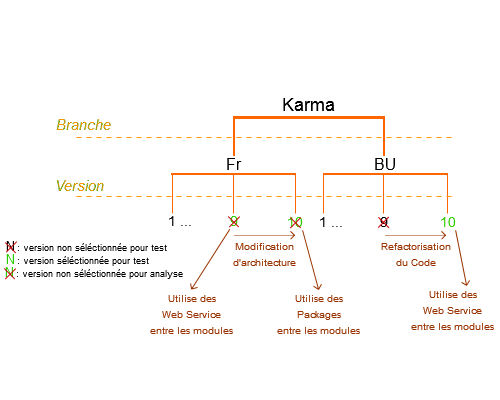
\includegraphics[scale=0.9]{./img/choix_karma.png}
    \caption{Choix de la version de \gls{karmag} à utiliser}
\end{figure}
\paragraph*{}Le but n’était pas d’étudier le fonctionnement de l’intégralité de \gls{karmag} mais uniquement les modules qui pouvaient être utiles. Marc DOUET m’a indiqué que le module qui semblait le plus approprié pour le projet était le module \gls{x69g}. J’ai donc commencé à compiler puis déployer chaque module \gls{x69g} des versions retenues, pour ensuite comprendre leur fonctionnement. Pour cette étape, je me suis mis en relation avec les équipes de développeurs de chacune des deux branches. Ils m’ont aidé avec les spécificités de compilation et déploiement de chaque version. Cette étape a permis non seulement de connaitre les contraintes d’environnement pour chaque version, mais également servi à comprendre comment le module \gls{x69g} communiquait avec un client \gls{cwmp} et la manière de l’utiliser selon les versions.
\paragraph*{} Finalement, il est apparu que la version 10 \gls{karmafrg} des modules \gls{comg} et \gls{x69g} ne peuvent pas se passer de la base de données de \gls{karmafrg}, ce qui rend cette version inutilisable. La version 9 de \gls{karmafrg} est complexe à compiler et ne possède aucune documentation pour configurer son environnement de déploiement. De plus, le code de la branche \gls{karmafrg} n’est pas très propre et non documenté, ce qui a permis d’éliminer ces deux versions, ne laissant que les versions 9 et 10 de \gls{karmabug}. Or la version 10 de \gls{karmabug} est une refactorisation de la version 9, la randant plus intéréssante que la version 9. Le code de la version 10 de \gls{karmabug} est correctement documenté, de même pour la configuration de l’environnement de déploiement et son installation. Ainsi, mon choix s’est porté sur le module \gls{x69g} de la version 10 de \gls{karmabug}. \\
\subsubsection{Analyse de faisabilité}
\paragraph*{}Après avoir identifié la solution technique que nous devions utiliser, il
fallait utiliser la version de \gls{x69g} afin de créer une première version de \gls{tink}. Bien entendu, cette première version ne servirait que de test, permettant uniquement des échanges de requête avec un client \gls{cwmp}, sans logique de test \gls{cwmp}. Cette phase d’analyse de faisabilité s’est déroulée de mi-janvier à mi-février 2016 et comportait plusieurs objectifs. Il est important de noter que contrairement à la précédente phase, celle-ci avait une date limite et devait être terminée pour mi-février 2016, c’est-à-dire à la fin de ma période entreprise. Cette date limite se justifie par le fait que ce travail allait servir de base pour Jean-Pierre ONA, qui devait arriver courant mars 2016, durant ma période d’école.
\paragraph*{}Le principal but de cette phase était bien évidemment de commencer un
premier travail d’adaptation du module \gls{x69g} de \gls{karmabug} pour nos besoins. Cela a consisté à comprendre les mécanismes d’interactions des différents packages et classes, afin de pouvoir générer des requêtes \gls{cwmp} autres que celles utilisées lors de la première phase, c’est-à-dire les méthodes impliquées dans l’initiation de la session \gls{cwmp}. Cela m’a demandé de me concentrer sur la manière d’utiliser ce module pour choisir les méthodes \gls{cwmp} envoyées à un client \gls{cwmp} lors d’une communication.
\paragraph*{}Un second objectif fut de déterminer quelles sont les méthodes \gls{cwmp}
que le module \gls{x69g} implémente et nous permet donc d’utiliser. Cette étape était cruciale puisqu’elle a permis de déterminer quels tests nous allions pouvoir faire, ou non, et avec quelle complexité nous pouvions accéder et formater ces méthodes \gls{cwmp}.
\paragraph*{}Un troisième objectif, dépendant des deux précédents, était de définir de
manière plus structurée le projet dans une première version du cahier des charges. Par la suite, il m’a également fallu réaliser une première version du dossier de spécification. Le dossier de spécification devait être uniquement constitué des premiers tests susceptibles d’être fait. Ces documents devaient également aider Jean Pierre ONA à prendre connaissance du projet plus facilement.
\paragraph*{}En somme, l’objectif global de cette phase était de définir ce que nous
allions faire lors de la réalisation, en ayant une première version de \gls{tink} capable d’envoyer des requêtes \gls{cwmp}.
\paragraph*{}Lors de la réalisation de cette étape, j’ai dans un premier temps cherché
à mieux comprendre le code de \gls{x69g}. Cela n’a pas été simple pour moi puisqu’il utilise plusieurs \gls{frameworkg} Java assez complexes en terme de prise en main, concept java mais aussi développement et configuration. J’ai donc régulièrement communiqué avec Eduard COJOCARU, qui a retravaillé le code de \gls{x69g} lors du passage de la version 9 à la version 10 de \gls{karmabug}. Par conséquent, il a une très bonne connaissance de ce module. J’ai par ailleurs été amené à rencontrer d’autres développeurs seniors pour qu’ils m’expliquent les concepts et le fonctionnement de certains mécanismes de ce code. Ce travail m’a permis de trouver par quel moyen un \gls{cpe} sait quelle interface interroger pour communiquer avec \gls{x69g}.
\paragraph*{} Quand j’ai eu une vision globale du module \gls{x69g} et compris le
fonctionnement de celui-ci, je me suis concentré sur la compréhension du processus de
détermination d’une réponse du module \gls{x69g} au \gls{cpe}. Pour cela, j’ai eu à retracer le parcours d’un message d’un \gls{cpe} arrivant sur ce module, jusqu’à l’envoi de la réponse. Ce travail de \gls{reverseg} m’a permis de remonter aux parties qui « parsent » les messages reçus, et plus important aux classes qui créent les messages \gls{cwmp} à envoyer au \gls{cpe}. Encore une fois, lors de cette étape, Eduard COJOCARU m’a indiqué et expliqué de nombreux mécanismes de \gls{x69g} impliqués dans cette communication avec le \gls{cpe}, ainsi que des mécanismes plus généraux de Java.
\paragraph*{}Lorsque j’ai su comment \gls{x69g} traite les messages \gls{cwmp} des \gls{cpe} et comment moi-même en envoyer dans l’ordre de mon choix, j’ai créé une première \gls{servletg} qui utilise le module \gls{x69g}. Cette \gls{servletg} avait pour but de communiquer avec un \gls{cpe} qui voudrait établir une session \gls{cwmp} et lui envoyer les requêtes \gls{cwmp} voulues. Cela m’a permis de mettre en pratique pour la première fois l’ensemble des connaissances acquises depuis le début de ce projet.
\paragraph*{}Une fois les tests de communication entre ma \gls{servletg} et le \gls{cpe} effectués, j’avais une meilleure vision des tests qu’il serait possible d’implémenter parmi la liste de ceux proposés par l’équipe qui les fait habituellement. Il s’agissait donc maintenant de rédiger et spécifier cette première suite de tests afin que Jean Pierre ONA, qui arriverait durant ma prochaine période de cours, puisse avoir une aide pour comprendre le projet plus facilement.
\paragraph*{}Parallèlement à ce travail effectué sur le module \gls{x69g}, nous avons
commencé à mettre en place la gestion de projet de manière agile. Cela s’est traduit pour ma part à lister sous forme de \gls{trackerg} l’ensemble des tâches à effectuer. J’ai par conséquent dû mettre à jour ces \gls{trackerg} au fur et à mesure que j’avançais dans la réalisation de la tâche qu’ils représentaient. J’ai également suivi une formation sur \gls{kanbang} et \gls{scrumg}, ainsi que sur l’utilisation d’un outil de gestion agile de projet interne à Orange. \\

\subsection{Méthode de projet}
\paragraph*{}Nous avons utilisé la méthodologie de projet agile durant la période de mars 2016 à août 2016. Après cette période j'étais le seul à développer l'application, il n'était donc plus utile de poursuivre ainsi. Néanmoins, nous avons continué à nous référer aux \gls{userstoriesg} décrites durant la période de présence de Jean-Pierre ONA. 
\paragraph*{}Après que Jean-Pierre ONA eut pris connaissance de l’objectif du projet, nous avons commencé à réfléchir puis décrire en détail les \gls{userstoriesg} desquelles ont découlé les différentes tâches qui, plus tard, ont constitué les différents \gls{sprintg}.
\paragraph*{}Nous avons opté pour des \gls{sprintg} de trois semaines, à la fin desquels une démonstration était attendue. Les \gls{sprintg} ont été définis au fur et à mesure. De plus, le fait que je ne sois pas toujours présent en entreprise a rajouté une contrainte supplémentaire au déroulement du projet et au contenu des \gls{sprintg}.
\paragraph*{}Tout au long des \gls{sprintg}s, des \gls{standupg} ont été réalisés afin que, quotidiennement, chacun indique aux autres membres de l’équipe sur quoi il allait travailler et quels étaient ses objectifs. Nous avons mis en place des points d’avancement une à deux fois par semaine afin de répondre aux problèmes qui pouvaient survenir, discuter de certaines solutions techniques, ou bien encore reprioriser certaines tâches. Le contenu des \gls{sprintg}s étaient également défini lors de réunions en début de \gls{sprintg}, où nous étions présents tous les quatre.
\paragraph*{}Comme dit précédemment, la méthodologie de projet en agilité a permis de nombreuses modifications tout au long du projet et sur différentes parties. Bien que les \gls{userstoriesg} n’aient pas été modifiées au cours du projet, les contenus des \gls{sprintg} et de la \gls{releaseg} d’août 2016 ont été fortement modifiés entre le début du projet et aujourd’hui. De même, l’architecture logicielle et le modèle relationnel de données ont été revus entre les différents \gls{sprintg} pour s’adapter au \gls{sprintg} qui suivait et à l’ajout de fonctionnalités que cela impliquait. Ces évolutions sont parfaitement inhérentes à la méthodologie de projet agile.
\paragraph*{}Le premier \gls{sprintg} n’a été débuté qu’une fois les questions d’architecture logicielle réglées pour une première version, et les spécifications sur les différents tests rédigées. Lors du premier \gls{sprintg} qui a débuté en mai 2016, le but était d’envoyer une suite de requêtes simples à tous les équipements qui viendraient interroger l’interface de l’outil de test. Il ne devait pas y avoir de vérification du contenu des réponses des équipements. Il y avait seulement la possibilité de créer des utilisateurs dans le portail et de leur associer des équipements. Lorsque ces équipements viendraient contacter l’interface de l’outil de test dédiée aux équipements, différentes requêtes et réponses seraient échangées. La sauvegarde de ces données impliquait la création d’un modèle relationnel de données qu’il a également fallu établir. De plus, lors de ce \gls{sprintg}, les modules constituant l’outil et la base de données devaient être déployés sur \gls{kermitg}. Ce \gls{sprintg} a donc été l’occasion de prendre en main \gls{kermitg} en allant interroger l’équipe en charge du développement et maintien de cet outil.
\paragraph*{}Les second et troisième \gls{sprintg}s n’ont concerné que le portail web
puisque je n’étais pas présent en entreprise. L’interface et le design ont été revus et différentes fonctionnalités d’ergonomie ont été rajoutées.
\paragraph*{} A mon retour en juillet 2016, nous avons lancé le quatrième \gls{sprintg}, qui devait initialement aboutir à une première version de la plateforme, qui permettait la création d’un utilisateur ; l’ajout d’équipements ; la création d’un plan de test ; et le déroulement de celui-ci lorsque l’équipement viendrait établir une session \gls{cwmp} avec notre outil. Cependant, nous avons revu l’architecture globale du logiciel, et avons, à la suite de réflexions communes, décidé de reprendre la manière dont communiquent les modules entre eux, lesquels peuvent dialoguer avec la base de données ; et de clarifier de nouveau les rôles de chacun entre Jean-Pierre ONA et moi-même. La fin de ce \gls{sprintg} a été reportée à mi-août 2016 avec une diminution du nombre attendu de tests réalisables, et une redéfinition plus propre de l’architecture logicielle, ce qui permettrait de reprendre le code plus facilement dans le futur.
\paragraph*{}Après le départ de Jean-Pierre ONA, nous avons arrêté d'effectuer des \gls{sprintg}s, tout en continuant de réaliser les différentes \gls{userstoriesg} que nous avions précédemment planifiées. \\

\subsection{Conception} 
\paragraph*{}Les différents points de conception ont été réalisés par Jean-Pierre ONA et moi-même, puis présentés et soumis à Matthieu ANNE et Marc DOUET, avant de pouvoir être implémentés. Il n'a pas été exigé de nous que nous proposions dès le premier \gls{sprintg} une architecture complète répondant à l'ensemble des problèmes techniques des futurs \gls{sprintg}. Au contraire, à chaque \gls{sprintg} nous devions  modifier, et réviser le cas échéant, ces points de conception\footnote{Les points de conception sont ceux présentés dans cette partie: Modèle relationnel de données, Architecture logicielle, Modélisation des test, Conception des tests} en analysant les nouveaux objectifs. En revanche, nous devions défendre et argumenter nos choix de conception à chaque révision et modification.
\paragraph*{}A la suite du départ de Jean-Pierre ONA en aout 2016, peu de modification au niveau de la conception de l'application ont été réalisées. Le cas échéant le procédé de validation a été le même.
\paragraph*{}La plus grosse partie de la phase de conception de l'outil à eu lieu durant la période de mars 2016 à juillet 2016. D'autres évolutions ont eu lieu au cours de la troisième année pour mettre en place de nouvelles fonctionnalités, ou en renforcer d'autre. Comme mentionné précédemment, nous avons travaillé en méthode agile, l'architecture logicielle et le modèle relationnel de données de l'application ont donc été fortement amenés à évoluer au fur et à mesure des \gls{sprintg}s, pour finalement être fixés à la fin de l'année 2016 à ce qui est présenté ci-dessous. \\
\subsubsection{Modélisation des tests}
\paragraph*{}Le but de cette plateforme étant de réaliser des tests d'implémentation \gls{cwmp} sur des équipements, il nous a fallu concevoir un modèle de test. Ce modèle doit faciliter l'ajout de nouveaux tests dans le futur, l'analyse des messages \gls{cwmp} reçu, et la génération des rapports de tests. Ainsi nous avons produits un modèle de test basé sur quatre couches hiérarchiques défini comme suis: 
\begin{itemize}
\item Un \texttt{Test Plan}, est un scénario testant un ensemble de fonctionnalités \gls{cwmp} sur un équipement donné, et aboutissant à la création d'un rapport de tests.
\item Un \texttt{Test} permet de vérifier l'implémentation d'une fonctionnalité \gls{cwmp} en particulier au travers d'un ou plusieurs échange avec l'équipement, durant un temps donné. Dans un \texttt{Test Plan}, il doit y avoir un ou plusieurs \texttt{Tests}. Un \texttt{Test Plan} est réussi uniquement si tous ses \texttt{Tests} le sont.
\item Un \texttt{Step}, correspond à un échange \gls{cwmp} avec l'équipement à tester. Un \texttt{Test} est composé d'une ou plusieurs \texttt{Steps}. Il comporte donc le nom de la méthode \gls{cwmp} attendu ou à envoyer à l'équipement. Un \texttt{Test} n'est réussi que si toutes ses \texttt{Steps} le sont aussi, et si elles sont faites dans le temps définis pour le \texttt{Test}.
\item Un \texttt{Parameter}, représente un paramètre envoyé dans une méthode \gls{cwmp}. Ils peuvent à la fois être donnés par l'utilisateur, mais aussi défini par défaut par Orange, selon ce qui doit être testé. Une \texttt{Step} peut avoir plusieurs paramètres comme aucun. \\
\end{itemize} 
\subsubsection{Modèle relationnel de données}
\paragraph*{}Le modèle relationnel de données sur lequel nous nous sommes arrêtés courant mars 2017 est formé de huit tables:
\begin{itemize}
\item \texttt{user}: Table permettant de sauvegarder les données utilisateur.
\item \texttt{device}: Table permettant à un utilisateur associé d'enregistrer un ou plusieurs équipements à tester.
\item \texttt{test\_plan}: Table permettant à un utilisateur de créer un scénario de tests à exécuter pour un équipement donné.
\item \texttt{test}: Table permettant de retenir un test composant un scénario de tests.
\item \texttt{message}: Table où sont stockés les messages générés par l'analyse d'un test, constituant le rapport d'un plan de test.
\item \texttt{test\_type}: Table stockant les différents type de test pouvant être sélectionnés par l'utilisateur lors de la création d'un plan de test. Il contient les caractéristiques de chaque test.
\item \texttt{step}: Table permettant de connaître les échanges \gls{cwmp} constituant un test donné. 
\item \texttt{parameter}: Table permettant de savoir quel(s) paramètre(s) passer à la méthode \gls{cwmp} qui sera envoyée à l'équipement.
\end{itemize}
%Import Images
\begin{figure}[!h]
    \center
    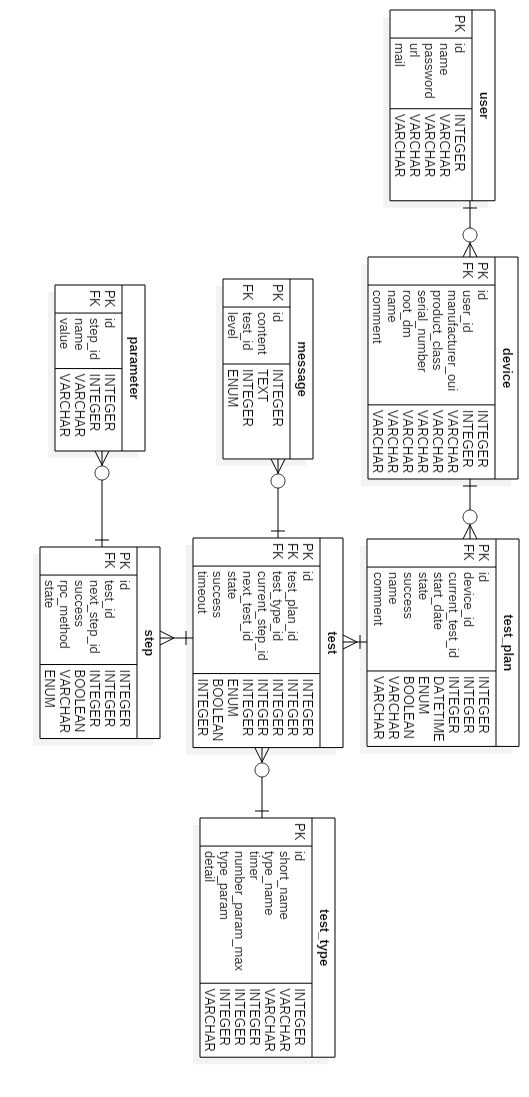
\includegraphics[scale=0.78]{./img/db_schema.png}
    \caption{Modèle relationnel de données}
\end{figure}
\paragraph*{}Ces tables forment quatre parties utilisées par les modules qui constituent l'architecture logicielle de \gls{tink}. La partie User, composée de la table user, la partie Device composée de la table device, la partie TestType composée de la table test\_type, et la partie Test composée des tables test\_plan, test, step, message et parameter. \\
\newpage
\subsubsection{Architecture logicielle}
\paragraph*{}Trois modules composent la plateforme \gls{tink}: GUI, TestManager et CWMP\_I. Ces trois modules sont indépendants les un des autres et communiquent uniquement par les \gls{api} qu'ils exposent. Ainsi ils ne partagent pas de dépendances et peuvent être déployés sur des serveurs d'applications différents. 
\begin{itemize}
\item \texttt{GUI}: Permet aux utilisateurs d'intéragir avec \gls{tink} à travers une \gls{ihm}. Ce module est responsable des interactions classiques tels que la création et modification d'un compte utilisateur, la création de test, la consultation et l'exportation de rapport de test, ou encore l'ajout d'un équipement à tester. Il peut communiquer avec les parties utilisateur, équipement et type de test de la base de données. Il a été décidé qu'il n'avait pas de besoin à connaître la logique de plan de test. De plus les informations sur les tests lui sont fournis par le module TestManager. 
\item \texttt{CWMP\_I}: Permet aux équipements de communiquer avec \gls{tink} à travers le module X69 qui provient directement des dépôts de \gls{karmabug}. Le fait que ce module soit importé par une dépendance permet de faciliter sa mise à jour en cas de développement de nouvelles fonctionnalités. Il n'a aucun besoin de communiquer avec la base de données car il est uniquement en charge des interactions \gls{cwmp} avec les équipements se présentant à \gls{tink}. Il récupère les méthodes et paramètres à envoyer aux équipements grâce aux \gls{api} du module TestManager. De la même façon, il envoi les messages \gls{cwmp} reçus et parsés par le module X69 au module TestManager pour leur analyse et la validation des tests. 
\item \texttt{TestManager}: Permet de connaître la logique de déroulement des tests. Il porte également l'intelligence pour la validation des tests. Il peut communiquer les résultats des tests au module GUI à travers ses \gls{api}, et envoyer de la même façon les méthodes et paramètres \gls{cwmp} au module CWMP\_I qui doivent être utilisés pour former les requêtes et réponses \gls{cwmp} envoyées aux équipements. Il n'a pas connaissance des utilisateurs et ne communique donc pas avec cette partie de la base de données.
\end{itemize}
Ci-dessous nous pouvons voir un schéma de l'architecture logicielle de \gls{tink} où sont présents les trois modules précédemment cités.
%Import Images
\begin{figure}[!ht]
    \center
    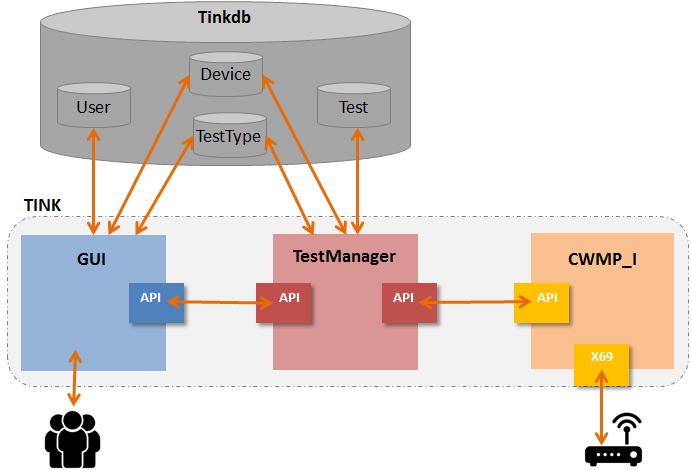
\includegraphics[scale=0.87]{./img/archi_logi.png}
    \caption{Architecture logicielle de TINK}
\end{figure}
\newpage

\subsubsection{Conception des tests}
\paragraph*{}La dernière partie de la conception de \gls{tink} a consisté à concevoir les tests qu'il devra être possible de réaliser. 
\paragraph*{}Nous devions dans un premier temps sélectionner les fonctionnalités à proposer aux utilisateurs de tester sur leurs équipements. Pour ce faire nous avons récupéré le plan de test qui est actuellement réalisé par les équipes en charge des tests de nouveaux équipements.   
\paragraph*{}Une fois les tests sélectionnés, j'ai déterminé quelles méthodes \gls{cwmp} utiliser pour réaliser chaque test; quels critères utiliser pour valider ou invalider les tests; quelles informations faire apparaître dans le rapport de chaque test. Une relecture du \gls{doctr069g} a été nécessaire afin d'interpréter les messages d'erreurs pouvant être renvoyés par l'équipement en cas d'échec de compréhension d'une requête \gls{cwmp}. Il a également été requis de regarder ce que \gls{karmag} et le \gls{doctr069g} attendent comme fonctionnalités et paramètres du \gls{datamodelg}.
\paragraph*{}Nous avons ainsi sélectionné douze tests. Pour chacun d'entre eux j'ai réalisé des diagrammes d'activités, détaillant à la fois comment ils seront implémentés, mais aussi à quels instants compléter le rapport de test. On peut voir en annexe un tableau descriptifs des douze tests sélectionnés. \\


\subsection{Réalisation}
\subsubsection{Travail en équipe}
\paragraph*{}L'équipe de travail sur ce projet a été amené à changer plusieurs fois tous au long de la réalisation du projet. Comme mentionné précédemment, de Octobre 2015 à mars 2016 nous étions trois, et mon travail était principalement axé sur la recherche de solutions techniques. Ainsi vis à vis des autres membres du projet, j'avais uniquement à présenter les résultats lors de points d'avancement hebdomadaire.
\paragraph*{}Le travail en équipe a fortement évolué et pris plus d'ampleur avec l'arrivée en mars 2016 de Jean-Pierre ONA. Il m’a été demandé d’encadrer ses activités et tâches lors de mes périodes en entreprise. Par conséquent, l’arrivée de Jean-Pierre ONA dans le projet en tant que développeur web et java, m’a demandé une adaptation dans mon organisation et les tâches que je devais accomplir ou lui donner. Nous avons choisi de travailler ensemble sur l’architecture logicielle de \gls{tink} en réalisant différentes évolutions de l’architecture qui, petit à petit, ont permis de définir le périmètre de chacun. A terme, chacun avait sa propre partie de l’architecture à
gérer, nous avons fait en sorte d’être cohérents dans nos choix.
\paragraph*{}Nos compétences techniques étant très différentes, cela nous a permis
d’établir clairement le périmètre de chacun une fois l’architecture choisie. Jean-Pierre ONA est plus axé développement java et web, tandis que je suis plus orienté sur la partie algorithmique, base de données, et possède une connaissance du protocole \gls{cwmp}. Ainsi, Jean-Pierre ONA a réalisé de la partie \gls{ihm} utilisateur, tandis que je me suis occupé de la partie interface équipement et réalisation/validation des tests. De plus, ayant une formation accès système, j’ai été en charge du déploiement et de la configuration système des serveurs d’applications et de la base de données sur \gls{kermitg}.
\paragraph*{}Durant les phases de développement des \gls{sprintg}s, nous avons régulièrement modifié le modèle relationnel de données afin de s’adapter aux exigences des \gls{sprintg}. Ces modifications ont nécessité une importante communication, dans un premier temps entre Jean-Pierre ONA et moi-même, puis avec Marc DOUET et Matthieu ANNE pour présenter les modifications et discuter ensemble les points bloquants. Ces révisions nous ont demandé une forte capacité d’adaptation, tant individuelle qu’organisationnelle. Les évolutions faites sur la base de données et sur l'architecture sont parfaitement inhérentes à la méthodologie de projet d’agilité.
\paragraph*{}À la suite du départ de Jean-Pierre ONA en août 2016, nous nous sommes de nouveau retrouvés à trois. Le travail était alors à la fois de continuer l'implémentation des fonctionnalités planifiées, mais également de récupérer et s'approprier le travail réalisé sur le module GUI par Jean-Pierre ONA. Matthieu ANNE et moi-même sommes montés en compétences sur ce module et y avons progressivement développés de nouvelles fonctionnalités.
\paragraph*{}Nous avons cessé de travailler sous forme de \gls{sprintg}, mais avons continuer de développer l'outil fonctionnalité par fonctionnalité, en faisant des points plusieurs fois par semaine. Nous n'avons pas apporté d'évolution majeure à l'architecture de \gls{tink}, ni repris la modélisation des tests. Cependant, nous avons adapté le modèle relationnel de données aux nouvelles fonctionnalités développées. Cela a pu se faire assez facilement grâce au travail réalisé précédemment. \\

\subsubsection{Développement}
\paragraph{Réalisation d'un \gls{poc}}
\paragraph*{}Nous avons choisi de coder \gls{tink} en Java J2EE, puisque nous souhaitions développer une plateforme en ligne. De plus, le module X69 de \gls{karmabug} que nous utilisons pour communiquer avec les équipements, est lui-même codé en Java. Nous avons donc décidé, pour des raisons de simplicité, de coder \gls{tink} en Java.
\paragraph*{}Le module X69 utilise plusieurs frameworks. Pour exposer une interface \gls{cwmp} en écoute pour les équipements, il utilise le framework CXF qui permet de simplifier l'utilisation et la gestion des \gls{servletg}. Afin de communiquer avec les équipements via le protocole \gls{cwmp}, et donc d'implémenter le protocole côté serveur, le module X69 utilise le framework Spring. Avant même de commencer le développement de \gls{tink}, il m'a fallu prendre en main ces frameworks, comprendre leur fonctionnement et leur utilisation dans le cas présent.
\paragraph*{}La première phase de développement a été faite durant la période de février à mars 2016\footnote{Cette phase a déjà été détaillé dans la partie "Analyse de faisabilité"}. Elle a permis de prendre en main les framework Spring et CXF, mais aussi de comprendre comment se greffer au code de X69 et récupérer les données provenant des messages \gls{cwmp} qu'il parse. A la fin de cette phase de développement un \gls{poc} de \gls{tink} a pu être réalisé. Cela consistait dans un premier temps à faire communiquer le module X69 avec un équipement. Dans un second temps je devais réussir à demander l'envoi de certaines méthodes \gls{cwmp} par X69 à l'équipement, et à en analyser les réponses.
\paragraph{Implémentation des bases}
\paragraph*{}La deuxième phases de développement c'est déroulée de mars à août 2016, avec la présence de Jean-Pierre ONA. Elle avait pour objectifs de réaliser une première version de \gls{tink}, avec la possibilité de se créer un compte sur la plateforme, tester des équipements, et avoir des rapports de tests détaillés et précis. Toutes ces fonctionnalités devaient être accessibles depuis la plateforme pour n'importe quel utilisateur. De plus, une majeure partie des tests devaient être présents. Afin de communiquer entre le code Java et la base de données, nous avons mis en place et pris en main le framework Hibernate. Aucun de nous deux ne connaissions ce framework, il nous a donc nécessité un certain temps pour monter en compétence dessus, mais cela nous a par la suite aidé. Cette phase a été particulièrement importante puisque nous avons développé à la fois la partie \gls{ihm}, la partie de logique de test\footnote{Par logique de test on entend: validation, déroulement et création des tests pour un équipement donné} et la communication avec les équipements. Cette phase m'a permis d'acquérir de solides bases en développement et en Java.
\paragraph{Évolution de TINK}
\paragraph*{}Enfin, la troisième et dernière phase de développement du projet, c'est déroulée durant l'ensemble de ma troisième année. Elle a principalement consisté à prendre en main la partie \gls{ihm} développée par Jean-Pierre. Elle a aussi permis l'ajout de nouvelles fonctionnalités et tests plus complexes, qui avaient été laissés de côté pour la première version par manque de temps. Jusqu'à présent seuls des tests réalisés sur une seule session \gls{cwmp} avaient été faits. De plus, les scénarios de test une fois lancés n'avaient pas de temps d'expiration, et nous ne pouvions pas les supprimer. 
\paragraph*{}L'une des fonctionnalités était de pouvoir placer un temps maximum d'exécution pour chaque test, modifiable par l'utilisateur. Cela a nécessité de prendre en main l'\gls{ihm}, mais également de modifier le modèle relationnel de données. Une autre fonctionnalité était de pouvoir récupérer l'intégralité du \gls{datamodelg} d'un équipement, cela n'est pas considéré comme un test mais comme une fonction supplémentaire. Nous avons voulu proposer aux utilisateurs la possibilité d'exporter un rapport de test dans le format .xls depuis l'\gls{ihm}. Cette nouvelle fonctionnalité a nécessité l'apprentissage de la librairie Apache POI, mais elle rajoute un réel plus pour les utilisateurs qui souhaitent nous transmettre leurs résultats. Il a également été rajouté la possibilité de supprimer des scénarios de test. Enfin, nous avons voulu réduire le nombre d'informations à apporter par un utilisateur pour ajouter un équipement, ainsi nous avons simplifié le formulaire d'ajout d'équipement et déduit les informations manquantes durant les échanges entre \gls{tink} et l'équipement. 
\paragraph*{}Une nouvelle version du module X69 a été développé par les équipes de \gls{karmabug}, avec l'implémentation de méthodes \gls{cwmp} supplémentaire. Cela a été pour nous l'occasion de tester l'intégration d'une nouvelle version du module X69, et d'évaluer concrètement l'impact sur le code que cela représente. L'import du module X69 étant uniquement réalisée par une dépendance Maven\footnote{Maven est un logiciel permettant, entre autre, de synchroniser les dépendances d'un projet Java avec les dépôts d'où elles proviennent. Il permet également de compiler le code Java selon certaines règles définies par le développeur}, cela a été transparent. Il nous a uniquement fallu prendre en main les fonctionnalités proposées dans cette nouvelle version. 
\paragraph*{}Au niveau des tests supplémentaires, avec l'ajout des temps d'expirations et la gestion du temps durant les tests, j'ai pu mettre en place des tests utilisant des calculs de temps. J'ai également implémenté des tests réalisés sur plusieurs sessions \gls{cwmp}. En tous nous sommes passés de sept à douze tests, couvrant ainsi à exception d'un test, l'ensemble des tests que nous nous étions fixés de faire initialement.
\paragraph*{}De plus, en parallèle du développement de l'ajout de nouvelles fonctionnalités, j'ai été amené à réviser et factoriser le code qui avait été produit lors de ma deuxième année. Le premier but de cette réorganisation de code était d'améliorer les performances. Le second but était de rendre plus propre et maintenable le code pour la suite de la vie de l'application. Cela m'a permis de renforcer mes compétences en développement Java, mais également d'apprendre des bonnes pratiques de code.
\paragraph*{} Enfin, avec le déploiement de l'application en production sur \gls{kermitg} en mars 2017, nous avons voulu rendre complètement automatique la génération de la base de donnée au démarrage des trois modules de \gls{tink}. Pour ce faire j'ai configuré le framework Hibernate via le code Java afin qu'il crée la base de données sur le serveur de base de données. Il crée également les tables du modèle relationnel par la suite, et les remplit avec les valeurs fixées dans le code. Ainsi, l'ensemble du déploiement, des modules à la base de données se fait automatiquement et ne nécessite aucune intervention extérieure.
\paragraph*{} L'ensemble de ces nouvelles fonctionnalités ont été implémentées sur la totalité de ma troisième année, et m'ont occupé une majeure partie de l'année. \\

\subsection{Lancement de l'application}
\paragraph*{}A partir de mars 2017, nous avons créé deux \gls{url}s, pour accéder via l'intranet et Internet à \gls{tink}, lançant ainsi en production l'application. Cela nous a lancé dans une nouvelle phase du projet. 
\subsubsection{Communication et présentation}
\paragraph*{}Afin d'avoir nos premier utilisateurs, il nous a fallu faire connaître notre plateforme. Nous avons donc communiqué et présenté \gls{tink}. Pour cela nous avons tout d'abord présenté l'application à notre département, puis plus largement à différentes équipes susceptibles d'être intéressées par l'utilisation de l'outil. Les présentations se sont déroulées en anglais et en français selon le public visé. Un texte de présentation de l'application a été rédigé en anglais par Matthieu ANNE, afin de le diffuser sur l'intranet et de le mettre sur la page d'accueil de l'application. 
\paragraph*{}Dès lors que des équipes en interne souhaitaient des informations sur un équipement, ou bien tester le comportement \gls{cwmp}, nous les redirigions vers \gls{tink} afin qu'ils puissent tester et connaître l'outil. Cela nous a permis d'avoir nos premiers utilisateurs et retours sur l'application. Certains membres de l'équipe ont également contribué à tester leurs équipements sur \gls{tink} et nous faire des retours sur les points d'améliorations et bugs rencontrés. \\

\subsubsection{Support utilisateur}
\paragraph*{}Dès lors que nous avons eu les premiers utilisateurs nous avons débuté leur support. Pour ce faire nous avons créé une adresse mail de contact que nous avons mis sur le site web. Nous avons également aidé certain utilisateur à trouver les informations nécessaires à l'ajout d'un équipement.
\paragraph*{}Une autre part du support utilisateur a été de récupèrer les retours sur l'application qui ont été fait, afin de lister les améliorations ou correctifs à apporter. Ces différentes révisions à apporter on ensuite étaient priorisées, avant d'être implémentées, certain n'ont pas encore pu être développées.
\paragraph*{}Nous avons également commencé à regrouper les questions qui nous ont été posées afin de créer plus tard une \gls{faq}. \\ 

\subsection{Bilan du projet}
\subsubsection{Difficultés rencontrées}
\paragraph*{}La première difficulté a été rencontré lors de la phase de recherche de solution, où j'ai eu étudier plusieurs versions de X69. Il a été nécessaire de définir l’utilisation et le rôle de X69 après son identification, afin dévaluer s’il répondait ou non à nos attentes. Cette phase a demandé une importante part de réflexion et d’analyse sur la manière dont nous pourrions utiliser les versions de X69 étudiées, dans le cas où elles étaient exploitables.
\paragraph*{}Une difficulté d'ordre techniques cette fois, portait sur la compréhension du code Java du module X69 composé de différents framework sur lesquels il m'a fallu monter en compétence. Cela c'est fait en grande partie de manière autonome, mais aussi avec l'aide de développeur senior qui ont pris le temps de m'expliquer le rôle et le fonctionnement de chaque framework, ainsi que certaine parties du code Java en lui-même. 
\paragraph*{}Le développement n'étant pas mon domaine, le fait de devoir concevoir, puis développer l'application de bout en bout, a été pour moi un réel défi à relever. Pour ce faire j'ai pu compter sur l'aide et les conseils de mes collègues, mais également m'appuyer sur certain cour de Java donnés aux élèves INFRES de la spécialité ED. 
\paragraph*{}L'encadrement et la répartition des tâches entre Jean-Pierre ONA et moi-même n'a pas toujours été simple. Notamment lors des semaines suivant son arrivé où nous avons rapidement vu qu'il nous fallait définir un périmètre à chacun, afin de ne pas confondre le travail entre nous.
\paragraph*{}Enfin, la rédaction du contenue des rapports de test a été une partie délicate du développement de \gls{tink}. En effet, les rapports devaient être à la fois minimales et apporter une réelle plus-value pour les utilisateurs. Cela a nécessiter de nombreuse réunion avec Matthieu ANNE, ainsi que des revus de diagramme d'activité mettant en évidence à quel instant écrire dans le rapport tel ou tel informations. \\

\subsubsection{Les suites pour TINK}
\paragraph*{}Le projet \gls{tink} est désormais en exploitation, mais de nombreuses fonctionnalités reste à développer. Afin qu'après mon départ d'autres développeurs puissent reprendre mon travail, j'ai rédigé une importante documentation servant de guide de développeur. Cette documentation, rédigée en anglais, reprend l'ensemble des points de conception de l'application, l'architecture, le détail de chaque module, package, class Java; le descriptif du modèle relationnel de données et de chaque attribut des tables le composant; le détails, le déroulement et la validation de chaque tests; la manière dont est hébergé \gls{tink} sur \gls{kermitg}; et donne des indications sur les différentes configurations systèmes à apporter aux serveurs d'application et de base de données. Ce document se compose également de l'ensemble des spécifications de l'application. La rédaction d'un tel document à nécessité près d'un mois et demi, mais sera très utiles afin de faire évoluer \gls{tink} par la suite.
\paragraph*{}De nombreuses évolutions sont envisagés pour le future de l'application. L'une d'entre elle est de pouvoir avoir une interface d'administration dans l'interface web avec des profils administrateur. Cette interface permettrait de visualiser l'ensemble des rapports de test de chaque utilisateur, ainsi que de supprimer des équipements, rapport de test et utilisateurs inactifs. Elle permettrait aussi de pouvoir rapidement consulter l'activité sur la palteforme aux travers de donnée statistiques
\paragraph*{}Avec l'arrivée de la nouvelle version du module X69, de nouvelle méthode \gls{cwmp} ont été implémentées. Il est donc prévu de créer les tests associés à ces nouvelles méthodes \gls{cwmp} afin d'enrichir la gamme de tests proposés par \gls{tink}.
\paragraph*{}Il serait également appréciable pour les utilisateur de ne plus avoir aucune informations à déclarer pour leur associé un équipement. Pour ce faire nous souhaitons grâce à \gls{kermitg} pouvoir générer une adresse \gls{url} par compte créé. Ainsi, l'utilisateur indiquerait à ses équipements de contacter \gls{tink} par cette \gls{url}, et dès lors que l'équipement arriverait sur cette \gls{url} il serait directement associé dans la liste des équipement de l'utilisateur en question. Le fait d'avoir une \gls{url} dédiés par utilisateur rajouterait également une couche de sécurité et de confidentialité pour les utilisateurs puisqu'ils seraient sur des canaux différents. 
\paragraph*{}Actuellement je fais office de référence sur l'application \gls{tink}, afin de procéder à mon transfert de compétences j'ai rédigé le document de guide de développeur, mais également différents documents de présentation des choix d'architecture et un dossier de spécification. J'ai également travailler avec Matthieu ANNE sur le support des premiers utilisateurs afin d'indiquer les marches à suivre pour consulter les journaux d'événements des serveurs d'application, accéder à la base de données, etc... \\

\subsubsection{Apport personnel}
\paragraph*{}Les compétences développées et renforcées au cours des deux ans passés sur la création de \gls{tink} sont nombreuses. Ce projet m’aura beaucoup apporté autant au niveau transverse que technique. Globalement, ce projet fut non seulement axé sur le développement, mais également sur le système, ce qui en fait un réel « plus » dans mon parcours d’apprentissage et pour mes futurs missions et projets.
\paragraph*{}Le fait d'avoir pu gérer de bout en bout la recherche de solution technique, la conception, le développement, la mise en production et le support des utilisateur m'a permis de développer des compétences sur l'ensemble des phases d'un cycle de vie d'un projet. \\
\paragraph{Compétences transversales développées}
\paragraph*{}Du point de vue des compétences transversales j'ai pu tout au long du projet augmenter mon autonomie et accroître mes responsabilités dans les choix de solutions techniques, puis sur les questions de conception.
\paragraph*{}L'encadrement et la répartition des tâches avec Jean-Pierre ONA m'a là encore permis de prendre davantage de responsabilité. De plus, cela a démontré la confiance de mon tuteur dans mon travail.
\paragraph*{}Durant les différentes étapes du projet j'ai eu à gérer l'avancement du projet, tous en devant respecter différentes contrainte de temps. Cela a eu lieu avant l'arrivée de Jean-Pierre ONA et durant les phases de réalisation des \gls{sprintg} qui devaient être fait en un certain nombre de jours. Cela m'a permis d'apprendre à gérer mon stress et mon temps.
\paragraph*{}La communication est l’une des compétences transverses qui a été la plus
sollicitée. Elle a été primordiale pour le bon déroulement du projet. Non seulement lors des différentes réunions de travail où j’ai non seulement été amené à présenter et justifier mes choix d’architecture pour ma partie, mais aussi pour réaliser ce même travail en binôme avec Jean-Pierre ONA lorsque cela relevait de l’architecture globale. La communication a été également très importante avant les phases de développement lors de la définition du périmètre pour éviter de développer des modules qui ne peuvent pas s’interfacer, ou redévelopper en double certaines parties de code entre Jean-Pierre et moi. La communication a aussi été importante pendant le développement, puisque nous devions nous mettre d’accord sur les services que nos modules exposaient l’un à l’autre, la manière d’interroger ces services, et comment traiter les informations reçues. Plus récemment, j'ai eu à présenter devant des équipe françaises et internationales l'application, ce qui là aussi à accru mes compétences en communication. Ainsi, par cette importante communication avec les différents membres de l’équipe du projet, j’ai pu grandement renforcer mes compétences en travail collaboratif. 
\paragraph*{}Les sujets abordés n’étaient pas les mêmes selon les personnes. Avec
Jean-Pierre ONA, cela relevait plus de points techniques et d’organisation entre nous. Avec Marc DOUET et Matthieu ANNE, j’ai bénéficié de leur expérience pour apprendre
d’avantage sur la gestion de projet, et sur la manière d’évaluer la durée et la complexité des tâches. En outre, ils m’ont avant tout permis de renforcer mes compétences d’analyse et d’évaluation d’une solution, face à une liste de besoins préétablie, ainsi que de pousser ma réflexion suffisamment pour ne pas s’arrêter sur la première solution. Cela m’a appris à m’assurer que la solution choisie couvre bien tous les cas, en prenant suffisamment de recul. De plus, du fait de la gestion de projet agile, nous pouvions très bien la revoir plus tard pour une solution plus optimale.
\paragraph*{}Lors des différentes réunions, que ce soit avec Jean-Pierre ONA ou pour
des parties qui me concernaient uniquement, j’ai été amené à rédiger plusieurs
présentations et supports afin d’avancer et argumenter mes choix techniques. Cela m’a
permis d’améliorer mes compétences de présentation et d’argumentation de choix.
\paragraph*{}Par ailleurs, lors du déploiement sur \gls{kermitg}, j’ai été amené à collaborer
avec l’équipe de \gls{kermitg}, pour qui nous avons entre autre servi de testeurs pour leur nouvelle version de leur service, puisque nous avons déployé sur la version beta de la nouvelle version de \gls{kermitg}. Ainsi, j’ai régulièrement remonté les bugs observés, renforçant mes compétences à travailler avec d’autres équipes ou services.
\paragraph*{}Le fait d’être en agilité impliquait que l’ensemble des tâches et problèmes rencontrés devait être journalisés, dans ce que l’on appelle des \gls{trackerg}, sur une plateforme de gestion de projet. Ainsi, quotidiennement je devais organiser les tâches à réaliser et mettre à jour les avancées effectuées sur les autres. Cela a permis d’améliorer mes compétences de priorisation et organisation.
\paragraph*{}Enfin, la communication régulière avec Edouard COJOCARU en anglais,
ainsi que la rédaction des \gls{trackerg}, documents de spécification, support de présentation, et guide pour développeur, en anglais, m’ont permis de renforcer davantage mon anglais technique. 
\paragraph*{}Cela a également était renforcé par les présentations faite en anglais à des équipes international. Durant ces présentations en anglais j'ai pu réaliser une démonstration de l'application, présenter le projet et \gls{tink}, ainsi que répondre aux différentes questions posées. L'ensemble a été correctement compris et le dialogue a pu ce faire sans difficultés de compréhension.
\paragraph{Compétences techniques développées}
\paragraph*{}Au-delà des compétences transversales, j’ai également développé et
renforcé des compétences techniques tout au long des deux années passées sur ce projet.
\paragraph*{}Tout d’abord sur la partie étude et développement, j’ai renforcé mes connaissances du langage de programmation Java acquises en première année. J’ai en effet collaboré avec des équipes de développeurs seniors, qui ont répondu à mes questions sur le code, et qui m’ont aussi expliqué et appris plusieurs principes sur Java, J2EE, les frameworkd Java tels que CXF, Spring et Hibernate, ou encore sur la compilation de projet via maven.
\paragraph*{}Concevoir l’architecture de l’application de bout en bout m’a permis de
fortement monter en compétence et développer mes connaissances sur les architectures n-tiers, et de manière générale, sur la conception d’architecture d’une application.
\paragraph*{}Le fait de pouvoir interroger des équipes de développeurs seniors m’a
aussi apporté beaucoup sur l’aspect architecture logicielle. Puisque l’architecture de \gls{karmag} et même l’architecture interne aux modules changent selon les versions, j’ai dû comprendre chacune d’entre elles, en particulier leur fonctionnement, pour faire mon choix. Elles m'ont également permis d'acfroître mes compétences tant au niveau génie logiciel que dans l’utilisation de Frameworks Java tels que Spring, CXF et Hibernate. Bien souvent les personnes qui m’ont aidé ne se sont pas juste contentées de me dire comment faire ce que je voulais, mais m’ont expliqué les mécanismes de fonctionnement de tels outils. Cela m’a permis de renforcer mes compétences en Java et en concepts de programmation.
\paragraph*{}Sur la partie système et réseaux, lors de ma collaboration avec l’équipe de \gls{kermitg}, j’ai été amené à développer des scripts d’installation pour leur client sur des machines Linux, puisque jusqu’à présent il n’y avait pas d’installation du client de \gls{kermitg} sur Linux. Cela m’a permis de renforcer mes compétences de scripting Linux.
Toujours avec l’équipe de \gls{kermitg}, j’ai servis de testeur en suivant certains de leurs nouveaux tutoriaux dont j’avais besoin pour le projet, mais qui n’avaient pas encore été utilisés. Dans le cas où je rencontrais des problèmes, j’ai apporté une correction ou des informations supplémentaires nécessaires pour la bonne réalisation des tutoriaux, renforçant davantage mes compétences en système Linux.
\paragraph*{}Bien que je connaissais déjà Docker grâce à mon auto formation faite suite au projet \gls{evolve} de deuxième année de l’école, la prise en main de \gls{kermitg}, m’a permis de renforcer mes compétences sur la conteneurisation et particulièrement sur Docker.
\paragraph*{}J’ai renforcé mes compétences en administration de serveur de base de
données MySQL et Serveur d’application Tomcat, puisque j’ai eu l’occasion de déployer et configurer ces deux serveurs dans le cadre du projet, en modifiant leur configuration à plusieurs reprises.
\paragraph*{} La modélisation du plan de test avec sa logique de validation et de
déroulement m’a permis de renforcer mes compétences en modélisation de processus.

\newpage
\section{Bilan de compétences} 
\subsection{Environnement professionnel}
\subsubsection{Connaissance de l'entreprise}
\paragraph*{}Lors de mon arrivée au sein de l'entreprise, une présentation des différents services avec lesquels j'étais susceptible de travailler m'a été faite. Cela m'a permis dans un premier temps d'avoir une connaissance partielle des ressources humaines avec lesquelles je serais amené à travailler tout au long de mes trois années de formation. Grâce à cette connaissance de l'environnement de travail, j'ai pu savoir qui contacter directement en cas de besoin dans de nombreuses situations. Comme je savais que certaines personnes avaient auparavant abordées des sujets similaires ou dans des domaines équivalents, j'ai pu obtenir davantage de connaissances pour les sujets sur lesquels j'allais être amené à composer. De la même façon, lorsque j'ai rencontré des points bloquants sur la partie technique, j'ai su quelles personnes contacter afin de pouvoir monter en compétences plus rapidement et  résoudre la difficulté.
\paragraph*{}Enfin, si au cours de ma première année j'ai souvent eu à contacter différentes personnes pour leur demander des informations ou de l'aide, j'ai vu durant la deuxième année l'inversion progressive des rôles. En effet, des personnes sont venues me demander des renseignements. \\
\subsubsection{Anglais et contexte international}
\paragraph*{}Mes activités et projets de première année ne m'ont pas permis d'interagir avec des équipes internationales. Cependant, lors de ma deuxième année j'ai été amené à travailler avec un membre d'une équipe de conception et développement roumaine. Ce travail en collaboration a eu pour conséquence de me faire monter en compétence non pas uniquement sur l'aspect technique, mais aussi sur mon anglais écrit, puisque nous échangions en anglais par écrit le plus souvent.
\paragraph*{}De plus, durant l'ensemble des trois années j'ai pu traiter et rédiger de nombreux documents en anglais, dossier de spécificaiton, guide de dévelopeur de \gls{tink} etc. Lors de mon arrivée au sein de l'équipe, il m'a été aussi demandé de lire plusieurs documents techniques concernant le domaine dans lequel j'allais évoluer et travailler. L'ensemble de ces documents était rédigé pour la majorité en anglais, ce qui fut pour moi l'occasion d'acquérir des notions en anglais technique. Dans un second temps, j'ai eu à rédiger des documentations et participer à la rédaction de wiki du projet \gls{tink}. Ces rédactions ont été un moyen de mettre en pratique les notions d’anglais précédemment acquises. Lors de la deuxième année il m'a été demandé de rédiger un cahier des charges ainsi qu'un dossier de spécification intégralement en anglais. Cela m'a ainsi permis de monter en compétence en anglais technique tout au long de ces deux ans. Enfin, lors de ma troisième année j'ai pu continuer de pratiquer mon anglais écrit en dialoguant avec l'équipe roumaine qui maintien la plate-forme où \gls{tink} est hébergé. De plus, j'ai eu a rédiger une documentation technique entiérement en anglais, servant de base au futurs dévéloppeurs qui seront amenés à reprendre la suite de \gls{tink}. De même, j'ai pu travailler mon anglais oral durant la troisième année où j'ai eu à présenter en anglais et réaliser des démonstrations de mon projet à différents membres d'équipe d'autre pays.\\

\subsection{Management}
\subsubsection{Travail en équipe et communication}
\paragraph*{}Les premières missions qui m'ont été confiées n'impliquaient pas de travail collaboratif. Je devais faire des rapports à mon tuteur, selon l'avancée du projet. Ce dernier supervisait alors mes missions, en me laissant toutefois déjà une importante autonomie. Lors de réunions ayant lieu toutes les deux semaines, je présentais mon avancée de manière plus synthétique au reste de l'équipe. J'ai ainsi pu acquérir des notions en communication, ainsi que dans les compétences de restitution et présentation orale.
\paragraph*{}C'est dans la seconde moitié de ma première année que j'ai pu travailler sur des missions impliquant d'autres collaborateurs. Ce fut pour moi l'opportunité d'apprendre à organiser mon travail en prenant en compte également celui de mes collègues. Pour ce qui est de l'aspect communication, cela m'a permis de renforcer mes compétences en relatant mon travail lors des points d'avancés, mais aussi en étant force de proposition lors des réunions de travail où j'exprimais mon opinion sur les solutions envisagées et proposais d'autres possibilités.
\paragraph*{}Mon attitude professionnelle et l'évolution de mes compétences en travail d'équipe et en  management ont conduit mon tuteur à me confier l'encadrement partiel d'un stagiaire de Master 2 sur la seconde moitié de ma deuxième année. Il m'a été demandé de l'encadrer durant mes périodes en entreprise en répartissant entre nous les tâches composant le projet sur lequel nous travaillons. Cet exercice m'a permis de renforcer davantage ma communication et ma gestion du travail en équipe, en planifiant des réunions et des points d'avancement, ainsi qu'en assignant des activités au stagiaire. Cet exercice s'est correctement déroulé et m'a permis de renforcer ma confiance en moi. Cela m'a également appris à organiser, découper et répartir le travail d'un même projet entre plusieurs ressources.
\paragraph*{}Mes compétences en communication ont pu être renforcées lors de la dernière année, puisque j'ai eu à réaliser plusieurs présentations de \gls{tink} en duo avec Matthieu ANNE. Ces présentations ont été faite à plusieurs type de public, nécessitant d'adapter son discours selon les connaissances sur le sujets des personnes présentes. \\
\subsubsection{Gestion du temps et du stress}
\paragraph*{}Les missions qui m'ont été confiées tout au long des six premiers mois de ma formation n'impliquaient pas de date limite de rendu de projet. J'ai cependant eu besoin d'organiser mon travail et gérer le temps que je passais sur chacune de mes activités. Tout au long de la première année mon travail fut partagé entre deux activités principalement. Même si ces activités n'incluaient pas toujours un travail en collaboration, cela a tout de même nécessité l'organisation et la planification de mes temps de travail et actions sur chacune de ces deux activités. Cela m'a permis d'acquérir des notions dans ma gestion du temps.
\paragraph*{}Ce n'est qu'à partir de la seconde moitié de ma deuxième année que des contraintes de date limite m'ont été imposées. Cela fut notamment le cas dans le projet qui a occupé l'intégralité des deux dernières années, où différents jalons avaient été définis soit initialement, soit au cours du projet. J'ai alors mis en place des outils d’organisation afin de gérer mon temps de manière plus efficace et renforcer encore mes compétences dans ce domaine. J'ai appris à estimer la priorité, la complexité et le temps de réalisation de différentes actions, dans le but d’estimer de la façon la plus efficace possible le temps de travail nécessaire à la réalisation de ces actions.
\paragraph*{}L'apparition des dates limites et des enjeux à finir une activité dans le temps imparti m'a permis d'apprendre à gérer également mon stress. \\

\subsection{Conduite de projet}
\subsubsection{Analyse des besoins}
\paragraph*{}Les premières missions qui m'ont été confiées à mon arrivée au sein de l'équipe n'impliquaient pas de réelle analyse des besoins. En revanche, à partir de la seconde partie de la première année, j'ai eu progressivement des projets nécessitant que je recueille des besoins, fonctionnalités et critères essentiels pour mener à bien mes projets. Dans un premier temps cela consistait essentiellement à poser les bonnes questions à mon tuteur, qui m'avait attribué le projet. Progressivement j'ai eu à réaliser des études de faisabilités afin de démontrer que mes solutions étaient viables, ou tout simplement pour sélectionner la solution la plus adéquate au problème posé.
\paragraph*{}Mon tuteur m'a confié progressivement des missions qui nécessitaient une réflexion plus approfondie sur la recherche de solutions techniques et sur l'analyse de besoins, à partir de la seconde partie de ma première année. Afin que je puisse réaliser ce travail correctement lors de ma deuxième année. L'une des phases de mon projet de deuxième année consistait justement à définir et décrire les besoins, puis réaliser une étude de faisabilité de la manière la plus autonome possible puisque mon tuteur souhaitait que je réalise ces étapes moi-même tout en étant capable d'argumenter mes choix. Le fait d'avoir eu à examiner et à décomposer le projet en intégrant différents paramètres m'a permis d'avoir une certaine prise de recul sur ce que l'on me demandait de réaliser. \\
\subsubsection{Planification et méthode de gestion de projet}
\paragraph*{}Dès ma première année j'ai eu à planifier mes activités. Mais c'est à partir de ma deuxième année que j'ai vraiment pu utiliser des méthodes de projet, notamment l'agilité avec les méthodes Scrum et Kanban. Ces dernières m'ont permis d'organiser et préparer au mieux mon projet et mon travail collaboratif, puisque de cette façon je savais où en étaient mes collaborateurs dans leurs tâches sur le projet. Le fait de mettre en place cette méthode de projet m'a permis d'apprendre à décomposer le travail et à pouvoir le répartir entre les différents membres de manière égale et la plus adéquate possible en fonction des compétences de chacun et des tâches à réaliser.
\paragraph*{}Monter en compétence sur la gestion de projet et sur la décomposition des tâches m'a aidé à planifier au mieux mon travail et avoir une meilleure visibilité sur celui-ci.
\paragraph*{}J'ai de plus été amené à rédiger un dossier de spécification pour mon projet de seconde année, constitué d'un cahier des charges ainsi que de plusieurs diagrammes UML. Cet exercice de rédaction permet d'avoir encore une fois une meilleure vue sur ce qui est attendu, de son contexte et des différentes étapes. Lors de la troisième année, j'ai réalisé plusieurs diagramme d'activité, classes et séquences permettant d'illustrer le fonctionnement de \gls{tink}, ce qui là aussi m'a permis d'avoir une meilleur vision sur le travail à réaliser sur un projet donné.\\

\subsection{Systèmes d'Information}
\subsubsection{Architecture logicielle}
\paragraph*{}Durant ma première année j’ai pu, dans le cadre du projet de première année, concevoir une application utilisant l’architecture logicielle \gls{mvc}. Cela m’a permis d'acquérir des notions dans le domaine de patron de conception. Mon tuteur m’a également encouragé à utiliser d'autre patron de conception lors de l’un de mes projets qui nécessitait que je conçoive une application depuis le dossier de spécification, nécessitant donc de concevoir son architecture.
\paragraph*{}Lors de ma deuxième année, mon tuteur m'a confié la conception, puis le développement, d'un outil plus complexe que ce que j'avais pu réaliser jusqu’à présent. Cela a nécessité de ma part de prendre connaissance de plusieurs types d'architectures logicielles existantes. À savoir l'architecture n-tiers; comprendre chacune de ces couches qui composent cette architecture; leurs rôles et leurs fonctionnements. De plus, j'ai eu besoin de comprendre comment faire communiquer les différents modules de cette architecture, tout en prenant en compte les contraintes et les besoins impliqués dans le projet. Cela a nécessité de ma part de questionner des collaborateurs, développeurs seniors, ayant un niveau de compétences avancé dans l'architecture de logiciels et le développement. Le fait d'avoir pu contacter des développeurs seniors m'a permis de monter en compétence et d'avoir une importante source de connaissances à disposition. J'ai également récupéré les cours donnés aux étudiants INFRES ED de deuxième année qui abordent ce sujet, ce qui m'a permis d'acquérir davantage de connaissances.
\paragraph*{}J'ai ainsi conçu l'architecture logicielle d'une application, basée sur une architecture n-tiers, tout en prenant en compte les évolutions futures et la maintenabilité de celle-ci. Cela m’a permis de monter en compétence dans les architectures logicielles.\\

\subsection{Logiciels}
\subsubsection{Conception et développement d'applications}
\paragraph*{}Lors de mon arrivée dans l’entreprise, mon tuteur m’a fait travailler sur l’étude d’un client embarqué développé en C. Cela dans le but de me faire monter en compétence en développement C, puisqu’il m’a fallu comprendre le fonctionnement de ce client  à l’aide de reverse-engineering. Cela avait aussi pour but de me donner des notions en conception d’applications, en devant essayer de comprendre comment ce client avait était conçu. Puis dans un second temps, le modifier afin d'étudier la complexité à rajouter des fonctionnalités. Cette seconde phase m'a permis de mettre en application mes compétences en développement C mais aussi en conception.
\paragraph*{}Dans la seconde partie de ma première année, afin d’acquérir des notions supplémentaires dans la conception d’application, mon tuteur m’a fait travailler sur la conception d’un outil doté de fonctionnalités simples. La conception de cette application avait pour second objectif de me faire rentrer davantage dans le domaine d’activité sur lequel j’allais travailler durant mes trois ans de formation, en utilisant des concepts de cet outil. Cela m’a permis de monter à la fois en compétence sur les aspects de bases de conceptions d’applications, mais également de renforcer mes compétences en développement, particulièrement sur le langage orienté objet Java.
\paragraph*{}Lors de ma deuxième année, il a été décidé de me faire concevoir et développer un outil plus complexe que l’application implémentée en première année. Ce projet a occupé ma deuxième et troisième année. De plus, le travail de conception a été réalisé en travail collaboratif avec un second collègue. J’ai également pu demander des conseils, des explications, et des aides à différents développeurs seniors pour la conception de cet outil. De plus le développement de celui-ci s’est effectué en Java et m’a permis de travailler avec de nombreux frameworks fréquemment utilisés et relativement complexes à prendre en main. Le fait d’avoir pu apprendre à utiliser ces frameworks m’a permis d’acquérir de solides bases et compétences en développement Java.
\paragraph*{}De part la conception, l’étude et le développement de ces différentes applications, dans les langages C et Java, j’ai pu monter en compétence dans la conception logicielle et le développement d’applications.\\

\subsection{Base de données}
\subsubsection{Création et implémentation de modèle de données}
\paragraph*{}Lors des projets de cours de première et deuxième année j'ai eu à concevoir des modèles de données. Un premier, pour le projet de création de site web effectué à Bristol. Et un second durant le projet de deuxième année qui nécessité la création d'un site web la encore. Cela m'a permis de renforcer mes compétences en conception de modèle de données, mais aussi en langage SQL, puisque leur création c'est fait sur des serveurs MySQL.
\paragraph*{}Lors du projet d'entreprise \gls{tink}, j'ai également eu à concevoir de manière agile, un modèle de données. Ce modèle a dû être revu et amélioré tous au long du projet. Là encore cela a été réalisé en SQL.
\paragraph*{}J'ai ainsi pu renforcer mes compétences en création de modèle de données tous au long de ma formation, autant en entreprise qu'en école. \\
\subsubsection{Gestion et administration de SGBD}
\paragraph*{}Les connaissances de gestion et administration de \gls{sgbd} ont été en premier acquises par les cours suivis en première année, puis renforcées en deuxième année. Cette fois-ci cela était pour des serveurs Oracle et non MySQL, permettant ainsi de voir les différences de ces deux types de \gls{sgbd}.
\paragraph*{}Les projets de première année et deuxième année précédemment sités m'ont également permis de monter en compétences en administration de \gls{sgbd}, mais MYSQL cette fois.
\paragraph*{}En entreprise, c'est par le projet \gls{tink} là encore, que j'ai pu renforcer mes compétences en administration de \gls{sgbd}, en particulier sur MySQL. J'ai pu créer différents comptes, leur attribuer des droits en conséquence, et également réaliser des procédures stockées. \\

\subsection{Systèmes et Réseaux}
\subsubsection{Administration et maintenance d'OS}
\paragraph*{}Depuis le début de ma formation je travaille la majorité de mon temps sur des machines Linux, ce qui favorise le développement de mes compétences d'administration \gls{os} Linux et le langage orienté \gls{os} associé. De plus, lors de ma première année j'ai eu à recréer un réseau opérateur dans le cadre de tests d'équipements. Pour cela il m'a fallu configurer différents services et serveurs, me permettant de renforcer mes compétences en administration de système. J'ai par ailleurs eu à configurer et déployer des serveurs d'applications dans le cadre de ma deuxième et troisième année, ce qui a là encore pu renforcer mes compétences dans ce domaine acquis une première fois lors de mon DUT, mais aussi lors des cours de deuxième année que nous avons pu avoir.
\paragraph*{}Durant les périodes d'école de ma deuxième année j'ai également pu monter en compétence en administration d'\gls{os}, tant Linux et Microsoft, grâce aux différents cours qui m'ont été donnés.
\paragraph*{}Tout au long des deuxième et troisième années, j'ai pu monter en compétence sur certaines technologies de conteneurisation. En premier lieu grâce à un auto apprentissage lors du projet d'école de deuxième année, où mon équipe et moi-même sommes montés en compétence sur LXC et \gls{dockerg}. Puis en entreprise, où ces connaissances ont pu être renforcées et réutilisées lors de l'hébergement de l'application du projet \gls{tink} basé sur \gls{dockerg}. \\
\subsubsection{Protocole de Communication}
\paragraph*{}Tout au long de ma formation, mon domaine d'activité en entreprise a nécessité une forte connaissance du protocole de communication client/serveur, nommé \gls{cwmp}. Ce protocole est une importante brique de l'ensemble de mes projets. Il m'a donc été nécessaire de monter rapidement en compétence sur ce protocole dès mon arrivée dans l'entreprise. L’apprentissage de ce protocole m'a permis d'accroître mes compétence dans mes connaissances des protocoles de communication.
\paragraph*{}Les différents cours suivis lors de ma deuxième et troisième année, en réseaux et en télécommunications, m'ont également permis de monter en compétence sur d'autre protocoles de communication, tels que les protocoles liés au réseaux mobiles. \\
 
\subsection{Axe d'amélioration}
\paragraph*{} Ainsi que l'on peut le voir en annexe avec le \textit{Tableau d'auto-évaluation de compétences}, il y a de nombreuses compétences qui n'ont pas pu être encore développées ou approfondies. Cela s'explique par les sujets couverts jusqu'à présent lors des cours proposés à l'école, ainsi qu'aux missions effectuées en entreprise, qui ne peuvent bien évidemment pas couvrir l'ensemble des domaines du référentiel de compétence. Il est donc normal de voir des compétences plus avancées que d'autres, puisque l'on ne peut pas travailler sur toutes. Toutefois, il me semble intéressant pour mon futur professionnel de renforcer davantage mes compétences dans les domaines de \textit{Systèmes et Réseaux}, \textit{Conduite de projet} et \textit{Systèmes d'Information}. Ce sont pour moi des domaines de compétences qui m'attirent et vers lesquels je souhaiterais davantage me tourner. \\

\subsection{Conclusion}
Comme nous avons pu le voir tout au long de cette partie, ma première année fut pour moi riche en matière d'acquisitions de bases et notions dans de nombreux domaines de compétences. La seconde année m'a permis de renforcer ces compétences en améliorant ma manière de travailler, d'appréhender un problème, ou encore de faire face à un problème. Durant cette deuxième année, j'ai pu acquérir de nouvelles compétences, qui ont été elles aussi renforcées durant ma dernière année. Ces différentes phases d'acquisitions des compétences de l'ingénieur tendent ainsi à me rapprocher davantage du statut d'ingénieur souhaité par l'école. Durant ma dernière année, j'ai pu progressivement évoluer comme référence en matière d'outils de test du protocole \gls{cwmp}. On vient désormais me demander des renseignements ou du support pour les tests d'équipements.

\newpage
\section{Conclusion}
\subsection{Atteintes des objectifs}
\subsection{Progression}
\subsection{Synthèse de parcours}


\newpage
%ANNEXE
\begin{appendix}
\chapter{RPC Method CWMP}
\begin{table}
	\begin{tabularx}{17cm}{|l|X|}
		\hline
		RPC Method & Description\tabularnewline
		\hline
		InformResponse & Permet à l'ACS de répondre à un Inform.\tabularnewline
		\hline
		GetParameterValues & Permet de récupèrer la valeur d'un ou plusieurs 				paramètre du \gls{datamodelg} passé en paramètre.\tabularnewline
		\hline
		SetParameterValues & Permet de modifier la valeur d'un ou plusieurs 				paramètre du \gls{datamodelg} passé en paramètre.\tabularnewline
		\hline
		Reboot & Permet à l'ACS de demander au CPE de redémarrer.\tabularnewline
		\hline
		FactoryReset & Permet à l'ACS de demander au CPE de se réinitialiser à l'état d'usine.\tabularnewline
		\hline
		ScheduleInform & Permet à l'ACS de demander au CPE de revenir initialiser une session TR-069 dans t seconds.\tabularnewline
		\hline
		Download & Permet à l'ACS de demander au CPE de télécharger un fichier, souvent un nouveau firmware.\tabularnewline
		\hline
	\end{tabularx}
	\centering
	\caption{Liste des RPC méthodes devant être implémentées par l'ACS.}
\end{table}
\begin{table}
	\begin{tabularx}{17cm}{|l|X|}
		\hline
		RPC Method & Description\tabularnewline
		\hline
		Inform & Permet au CPE d'initier une session TR-069.\tabularnewline
		\hline
		GetParameterValuesResponse & Permet au CPE de répondre à un 						GetParameterValues en indiquant la/les valeur(s) du/des paramètre(s) 				demandé(s) par l'ACS.\tabularnewline
		\hline
		SetParameterValuesResponse & Permet au CPE de répondre à un 						SetParameterValues en indiquant si la demande a pu être réaliser.\tabularnewline
		\hline
		RebootResponse & Permet au CPE d'acquitter l'ordre de redémarrage.\tabularnewline
		\hline
		FactoryResetResponse & Permet au CPE d'acquitter l'ordre de réinitilisation à l'état d'usine.\tabularnewline
		\hline
		ScheduleInformResponse & Permet au CPE d'acquitter l'ordre de ScheduleInform.\tabularnewline
		\hline
		DownloadResponse & Permet au CPE d'acquitter l'ordre de Download.\tabularnewline
		\hline
	\end{tabularx}
	\centering
	\caption{Liste des RPC méthodes devant être implémentées par le CPE.}
\end{table}

\chapter{Liste des tests de TINK}
\begin{table}
	\begin{tabularx}{17cm}{|l|X|}
		\hline
		Test & Description\tabularnewline
		\hline
		TR-069 Init Session & Vérifie l'initiation d'une session \gls{cwmp} par le \gls{cpe}\tabularnewline
		\hline
		GetParameterValues Mandatory & Vérifie la bonne construction de GetParamaterValuesResponse et la présence des paramètres suivants, requis par \gls{karmag}: 
		\begin{itemize}
		\item ManagementServer.ConnectionRequestURL
		\item DeviceInfo.ProductClass
		\item DeviceInfo.ProvisioningCode
		\item DeviceInfo.ManufacturerOUI
		\item DeviceInfo.SerialNumber
		\end{itemize}		\tabularnewline		
		\hline
		GetParameterValues Custom & Equivaut au précédant test, mais la possibilité pour l'utilisateur de demander un GetParameterValues sur n'importe quel paramètre de son choix.\tabularnewline
		\hline
		SetParameterValues Mandatory & Vérifie la bonne construction de SetParamaterValuesResponse et la présence du paramètre suivant, requis par \gls{karmag}, DeviceInfo.ProvisioningCode\tabularnewline
		\hline
		SetParameterValues Custom & Equivaut au précédant test, mais la possibilité pour l'utilisateur de demander un SetParameterValues sur n'importe quel paramètre de son choix.\tabularnewline
		\hline
		UpdateConfiguration Mandatory & En plus d'envoyer un SetParameterValues, on vient ensuite vérifier le contenue du paramètre avec un GetParameterValues pour contrôler qu'il a été correctement mis à jour. Les paramètres à tester et requis par \gls{karmag} sont: 
		\begin{itemize}
		\item ManagementServer.PasswordConnectionURL
		\item ManagementServer.UserConnectionURL
		\end{itemize} \tabularnewline
		\hline
		UpdateConfiguration Custom & Equivaut au précédant test, mais la possibilité pour l'utilisateur de demander le test sur n'importe quel paramètre de son choix.\tabularnewline
		\hline
	%COUPER LE TABLEAU EN DEUX ICI !
		\hline
		\end{tabularx}
	\centering
	\caption{Liste des tests proposés par TINK (part 1/2)}
\end{table}

\begin{table}
	\begin{tabularx}{17cm}{|l|X|}
		\hline
		Test & Description\tabularnewline
		\hline
		Reboot & Vérifie la bonne construction d'un RebootResponse et que le \gls{cpe} parvient bien à redémarrer. Le \gls{cpe} doit contacter son \gls{acs} au redémarrage.\tabularnewline
		\hline
		Factory Reset & Vérifie la bonne construction d'un FactoryResetResponse et si le \gls{cpe} est capable de réinitiliser ses paramètres à l'état d'usine. \tabularnewline
		\hline
		Schedule Inform & Vérifie la bonne construction d'un ScheduleInformResponse et si le \gls{cpe} est capable dans un délais donné à plus ou moins cinq secondes. \tabularnewline
		\hline
		Connection Request & Vérifie si le \gls{cpe} est capable de revenir après la fermeture de session \gls{cwmp} et l'envoie d'un \gls{http} get de la part de son \gls{acs}. \tabularnewline
		\hline
		Periodic Inform & Vérifie si le \gls{cpe} peut revenir périodiquement à un interval de temps donné, à plus ou moins cinq secondes. \tabularnewline
		\hline
	\end{tabularx}
	\centering
	\caption{Liste des tests proposés par TINK (part 2/2)}
\end{table}


\chapter{Tableau d'auto-évaluation de compétences}
%Import Images
\begin{figure}[!ht]
    \center
    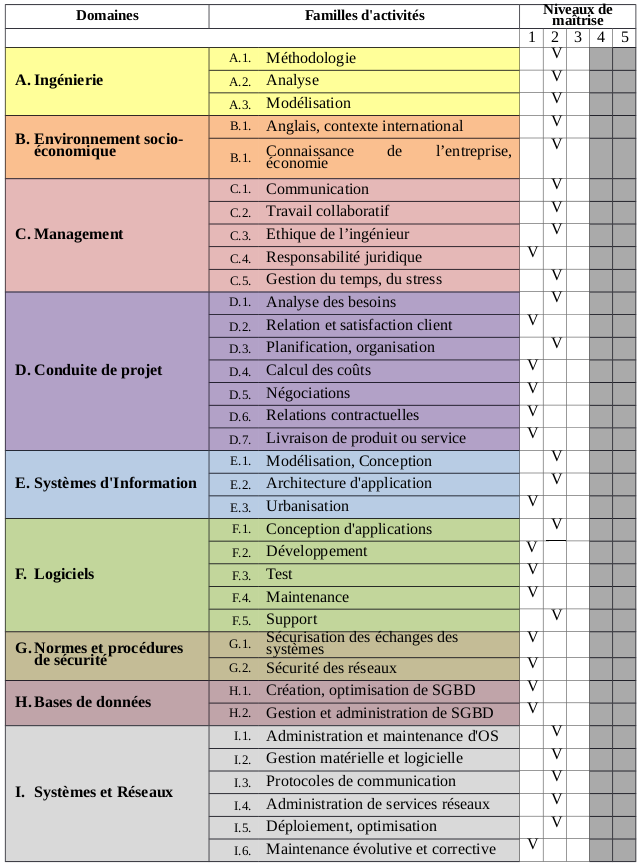
\includegraphics[scale=0.9]{./img/tableau_cpt.png}
    \caption{Tableau d'auto-évaluation des compétences}
\end{figure}

\end{appendix}

\newpage
\printnoidxglossary[type=main]

\end{document}
